%\section{Introduction}\label{sec:introduction-results}
%The following experiments are intended to be running for the use case
%which uses rule based matcher.

\section{Kafka Streams on Java 11}\label{sec:kafka-streams-on-java-11}

\begin{figure}[H]
    \centering
    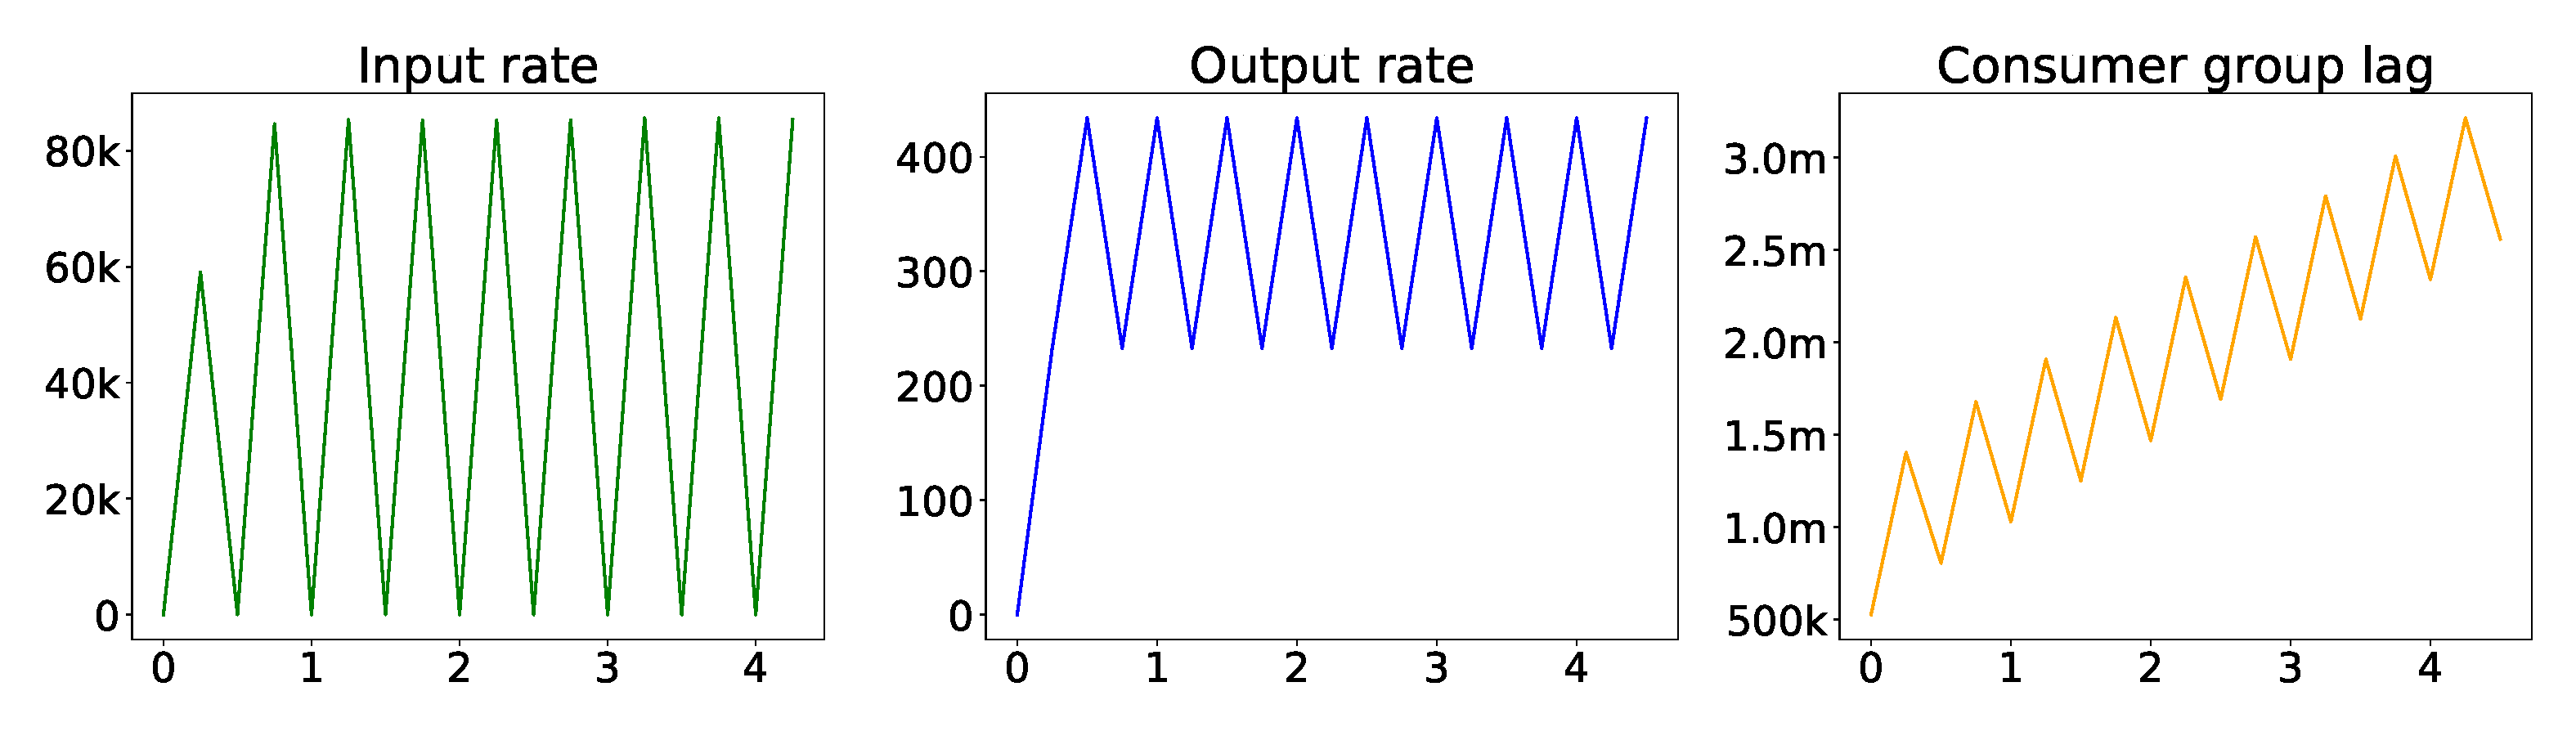
\includegraphics[width=1\textwidth]{figures/k-streams-java-11-replicas-10}
    \caption{Benchmark parameters: input MPS = 50k, replicas = 10, selectivity = 0.00002, rules = 10000. \\
    Consumer group regression slope: 446065.}
    \label{fig:k-streams-java-11-replicas-10}
\end{figure}

\begin{figure}[H]
    \centering
    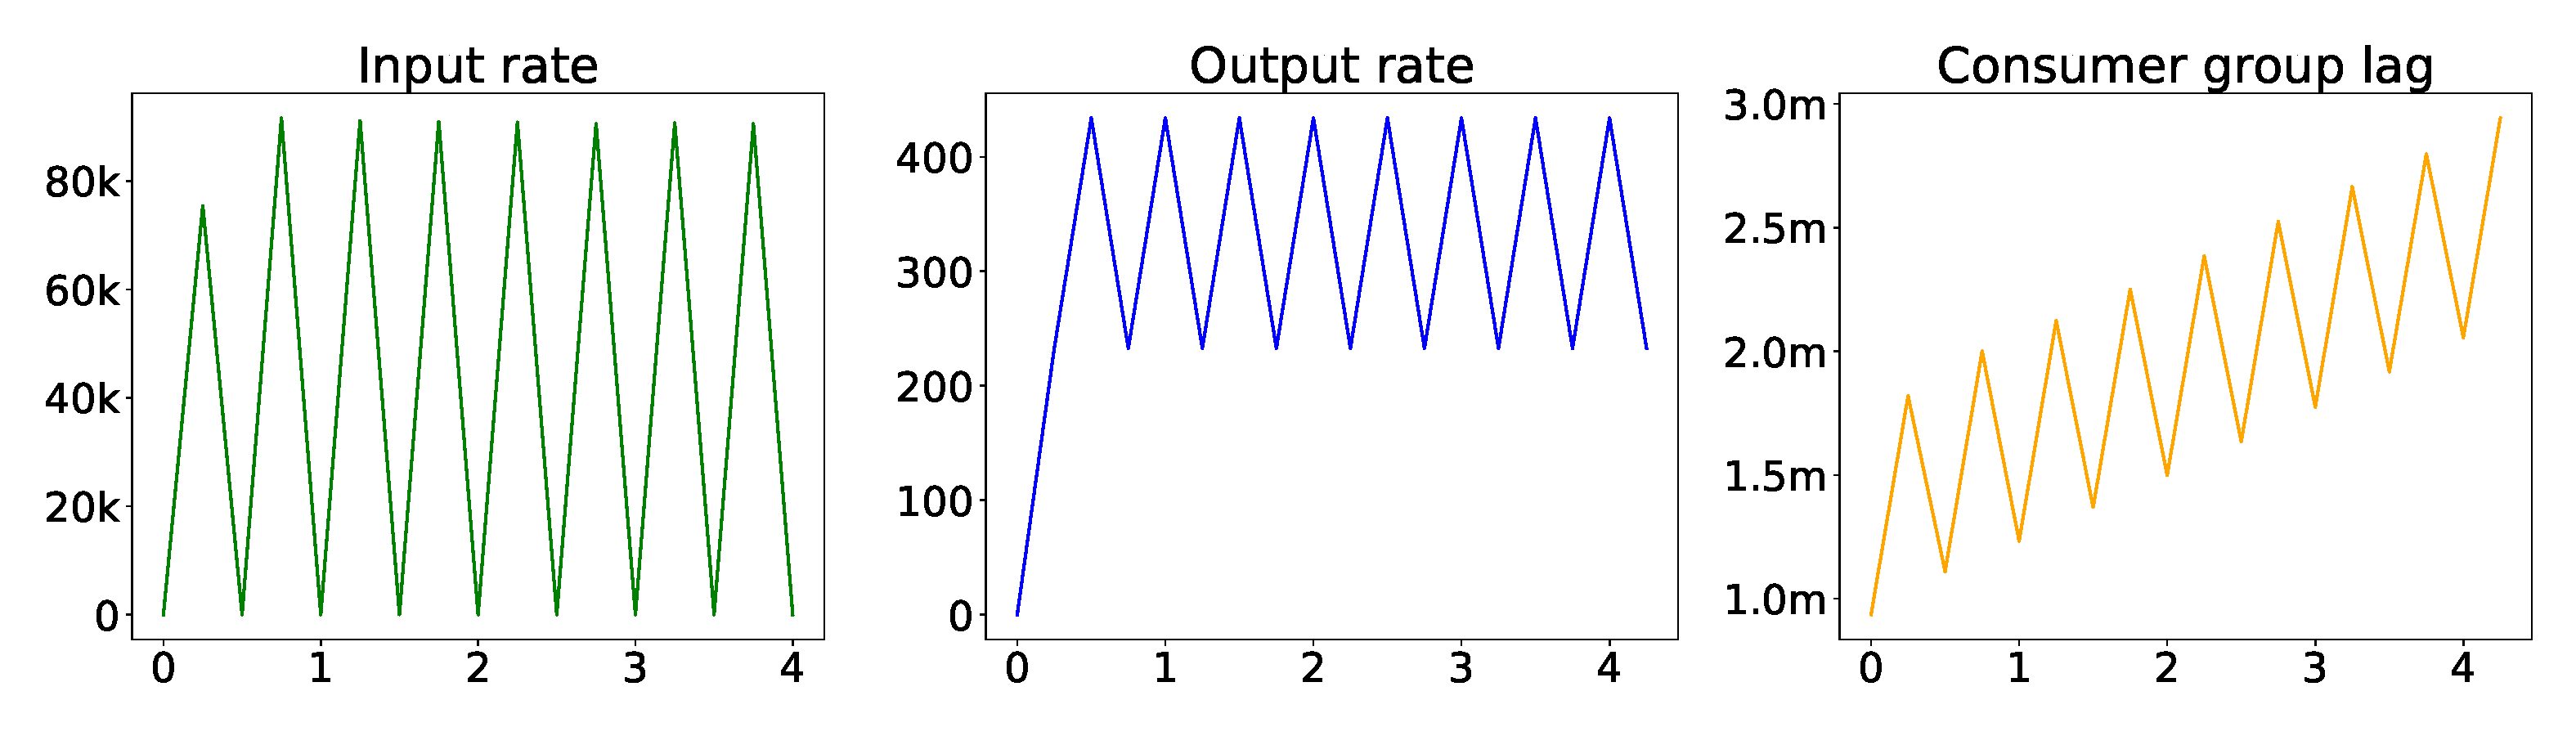
\includegraphics[width=1\textwidth]{figures/k-streams-java-11-replicas-11}
    \caption{Benchmark parameters: input MPS = 50k, replicas = 11, selectivity = 0.00002, rules = 10000. \\
    Consumer group regression slope: 305243.}
    \label{fig:k-streams-java-11-replicas-11}
\end{figure}

\begin{figure}[H]
    \centering
    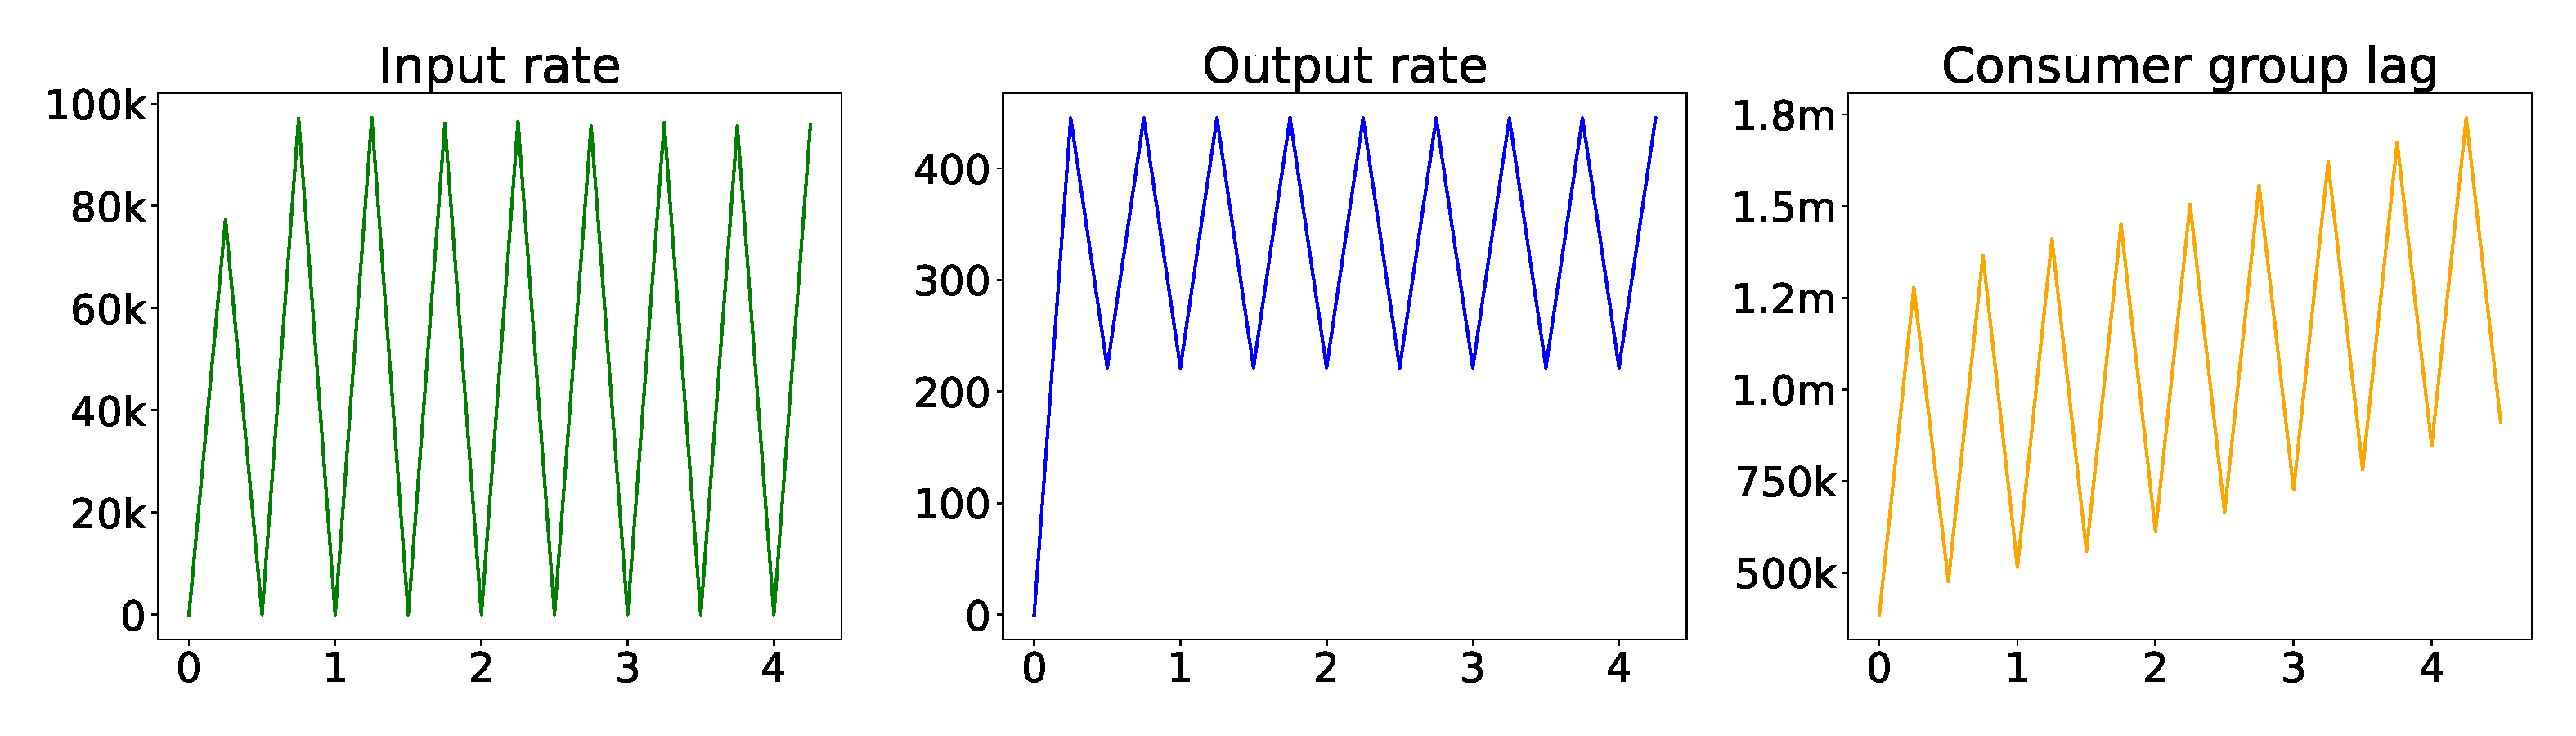
\includegraphics[width=1\textwidth]{figures/k-streams-java-11-replicas-12}
    \caption{Benchmark parameters: input MPS = 50k, replicas = 12, selectivity = 0.00002, rules = 10000. \\
    Consumer group regression slope: 110825.}
    \label{fig:k-streams-java-12-replicas-12}
\end{figure}

\newpage

\section{Kafka Streams on Java 21}\label{sec:kafka-streams-on-java-21}

\begin{figure}[H]
    \centering
    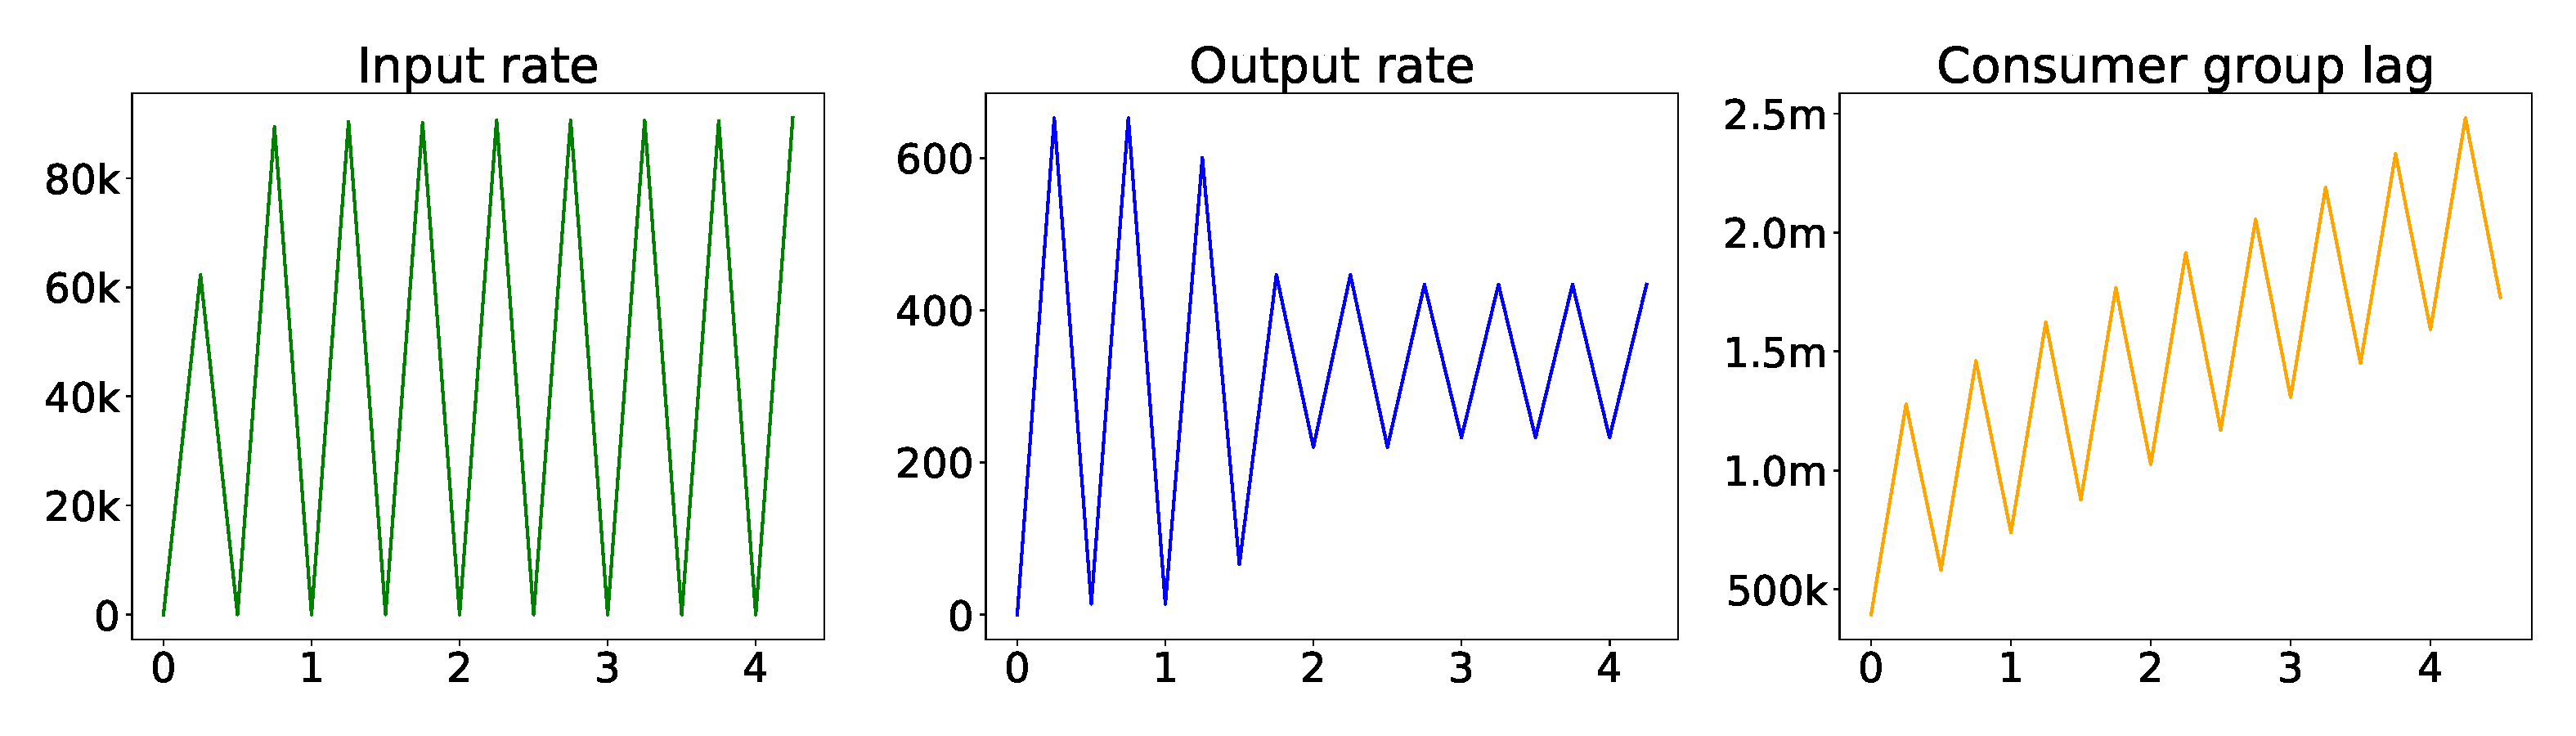
\includegraphics[width=1\textwidth]{figures/k-streams-java-21-replicas-10}
    \caption{Benchmark parameters: input MPS = 50k, replicas = 10, selectivity = 0.00002, rules = 10000. \\
    Consumer group regression slope: 293043.}
    \label{fig:k-streams-java-21-replicas-10}
\end{figure}


\begin{figure}[H]
    \centering
    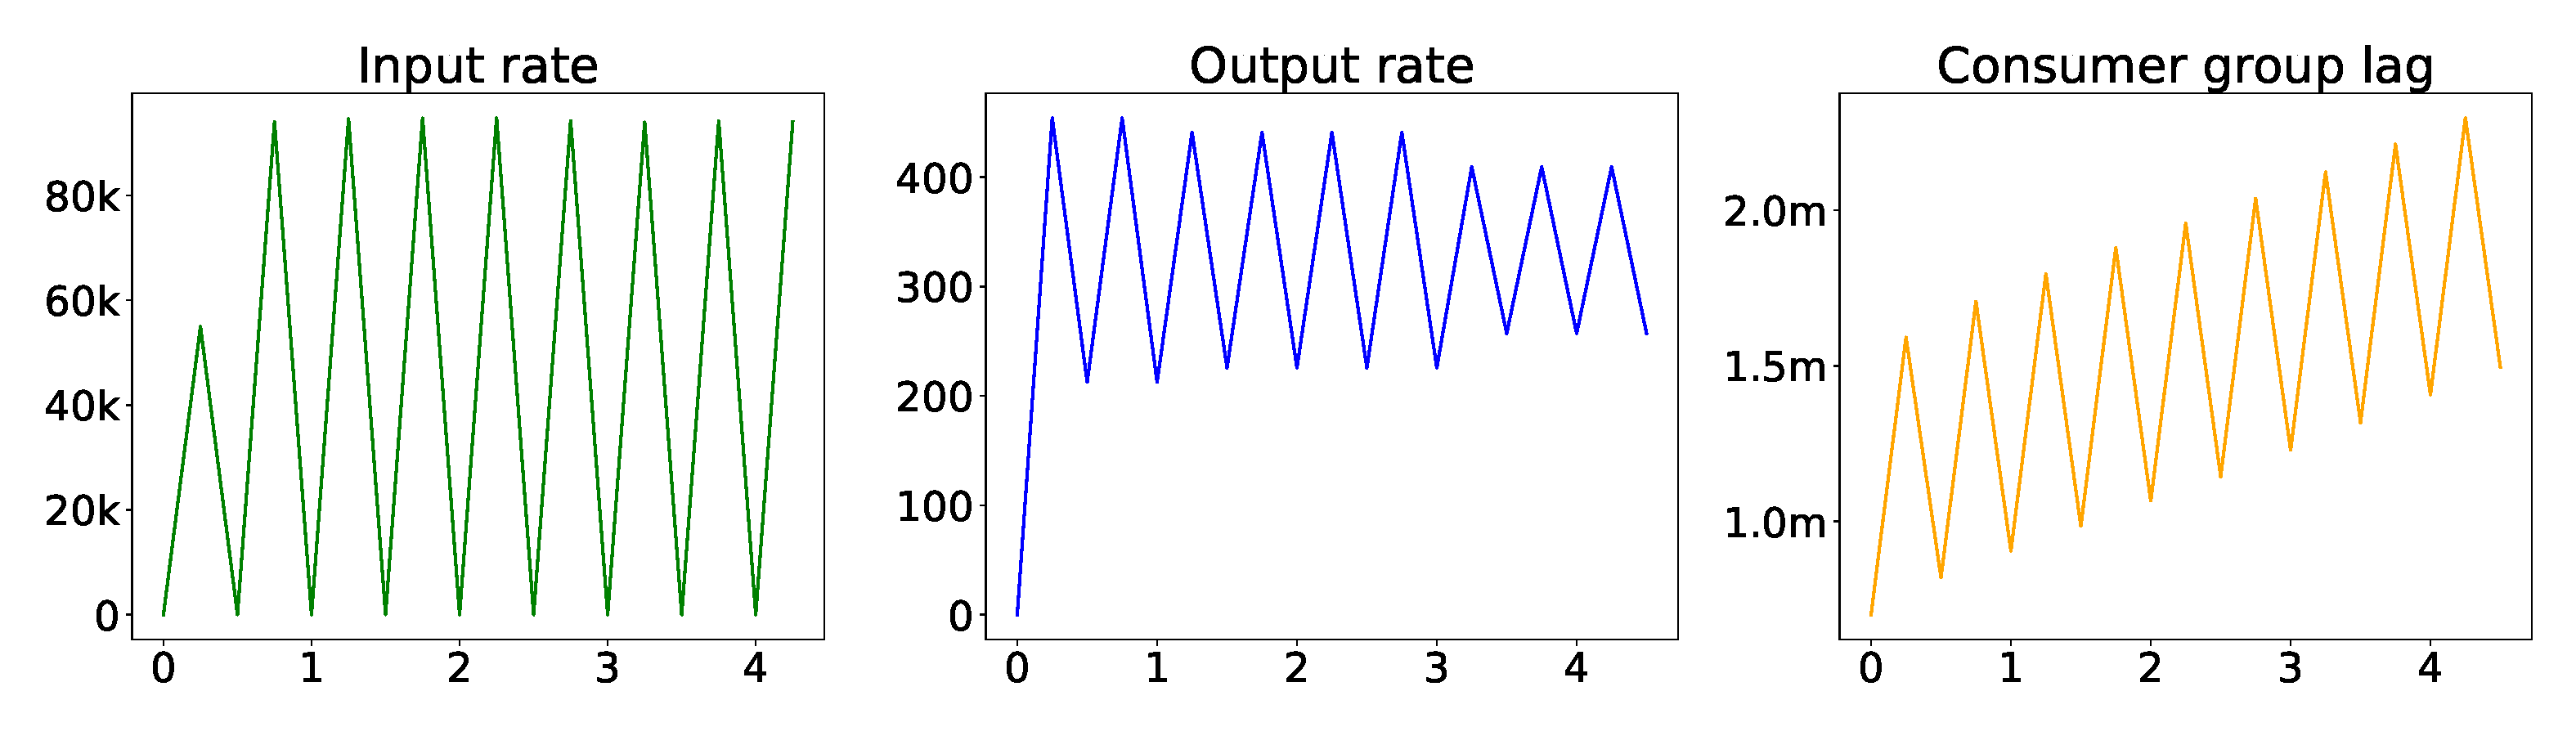
\includegraphics[width=1\textwidth]{figures/k-streams-java-21-replicas-11}
    \caption{Benchmark parameters: input MPS = 50k, replicas = 11, selectivity = 0.00002, rules = 10000. \\
    Consumer group regression slope: 171481.}
    \label{fig:k-streams-java-21-replicas-11}
\end{figure}

\begin{figure}[H]
    \centering
    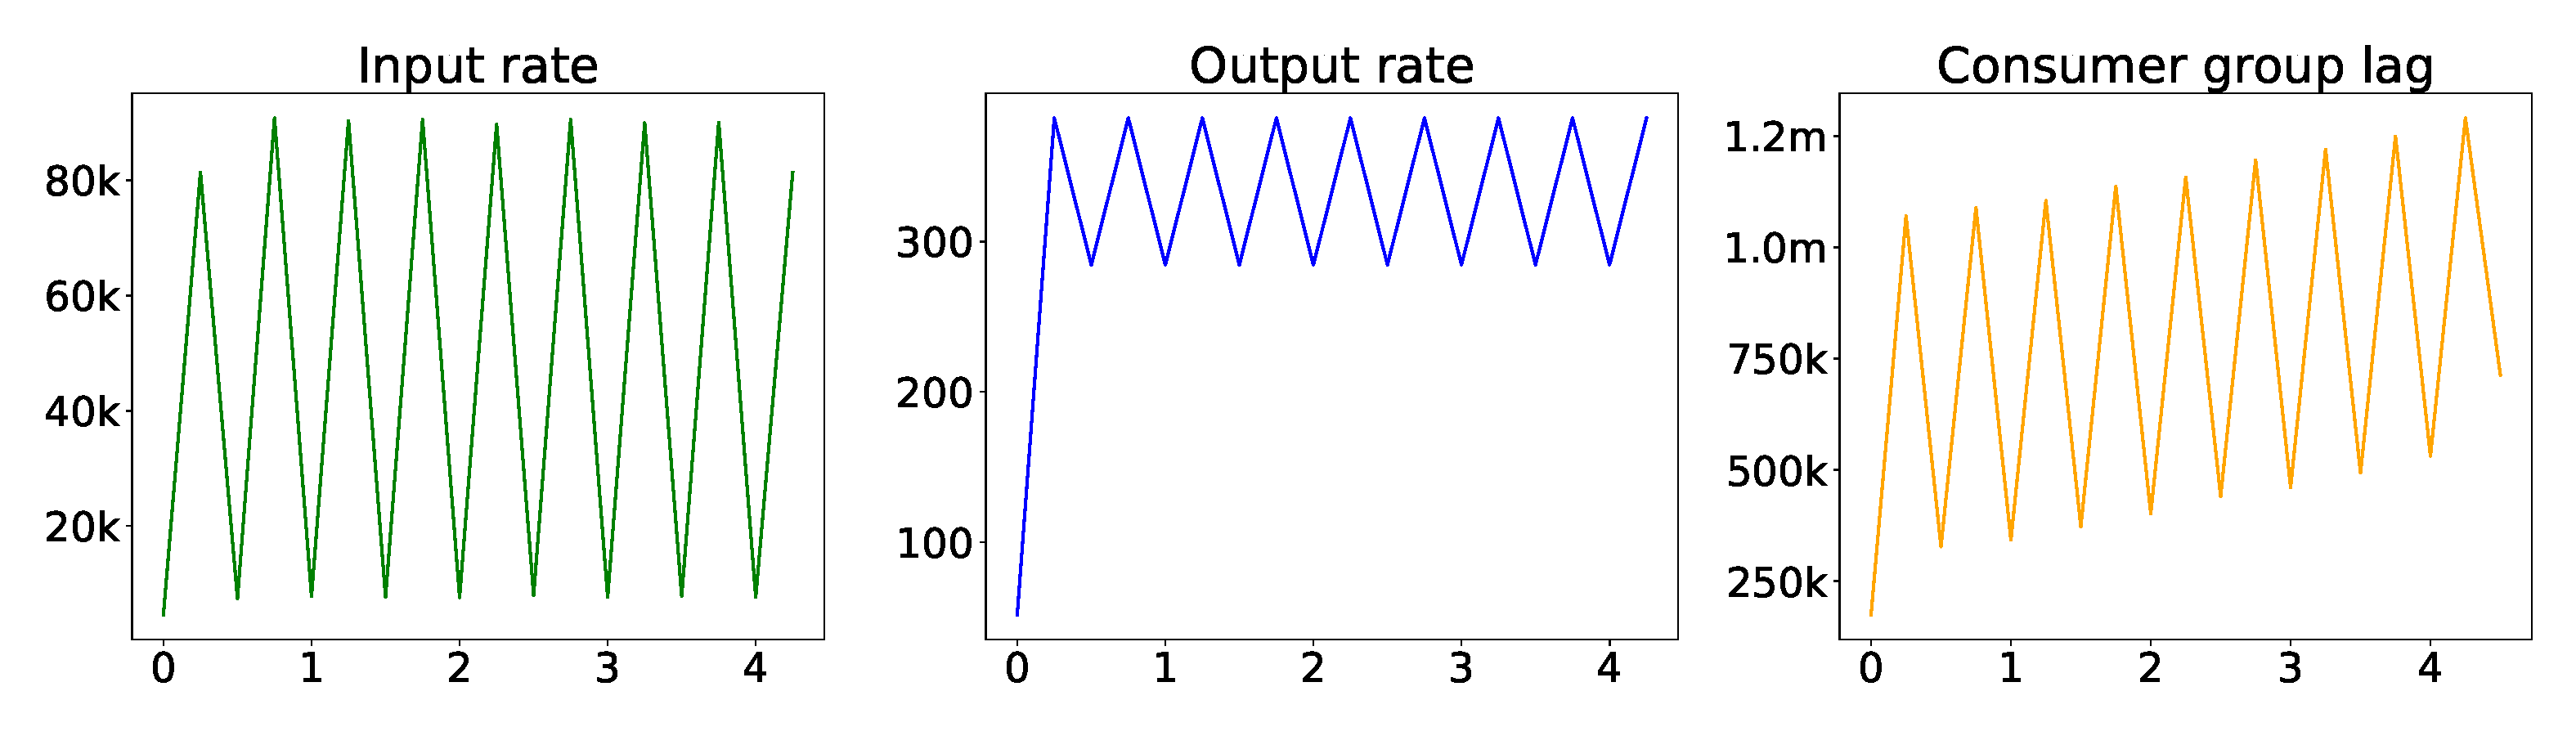
\includegraphics[width=1\textwidth]{figures/k-streams-java-21-replicas-12}
    \caption{Benchmark parameters: input MPS = 50k, replicas = 12, selectivity = 0.00002, rules = 10000. \\
    Consumer group regression slope: 74647.}
    \label{fig:k-streams-java-21-replicas-12}
\end{figure}


\newpage

\section{Kafka Streams on Java 21 with Generational ZGC}\label{sec:kafka-streams-on-java-21-with-generational-zgc}

\begin{figure}[H]
    \centering
    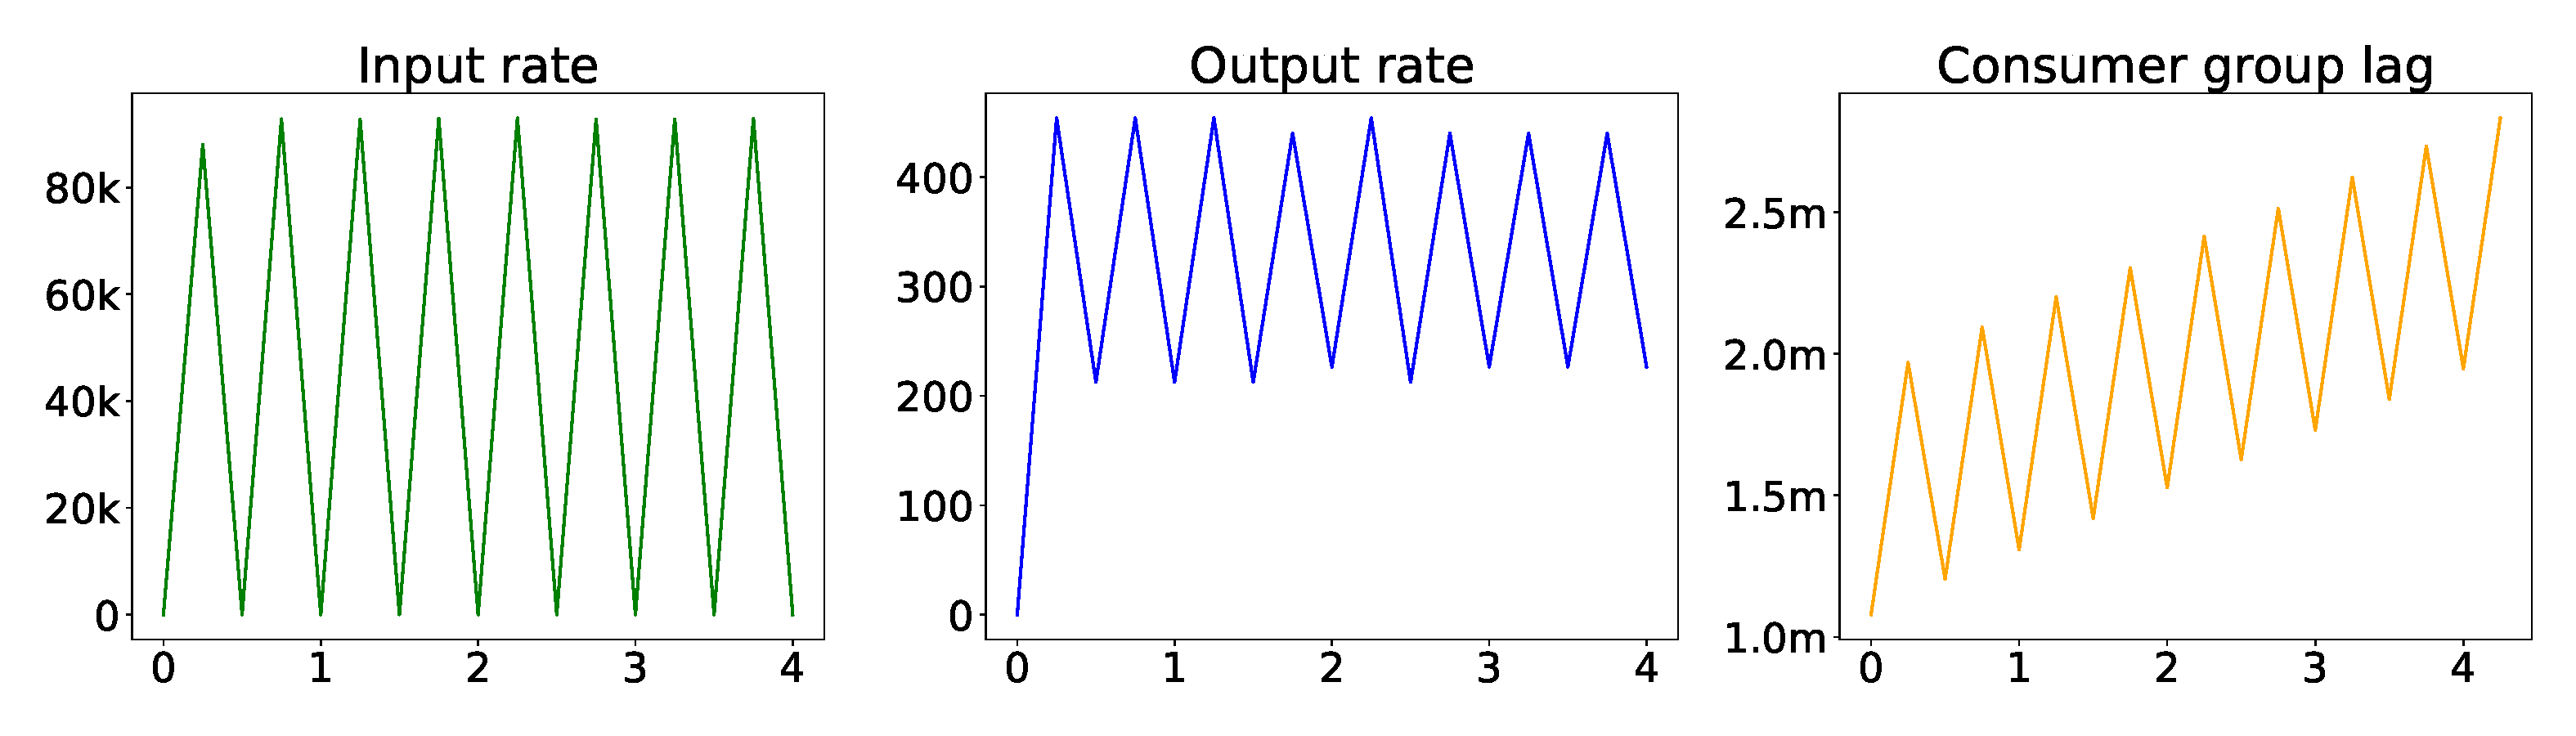
\includegraphics[width=1\textwidth]{figures/k-streams-java-21-new-gc-replicas-10}
    \caption{Benchmark parameters: input MPS = 50k, replicas = 10, selectivity = 0.00002, rules = 10000. \\
    Consumer group regression slope: 245290.}
    \label{fig:k-streams-java-21-new-gc-replicas-10}
\end{figure}


\begin{figure}[H]
    \centering
    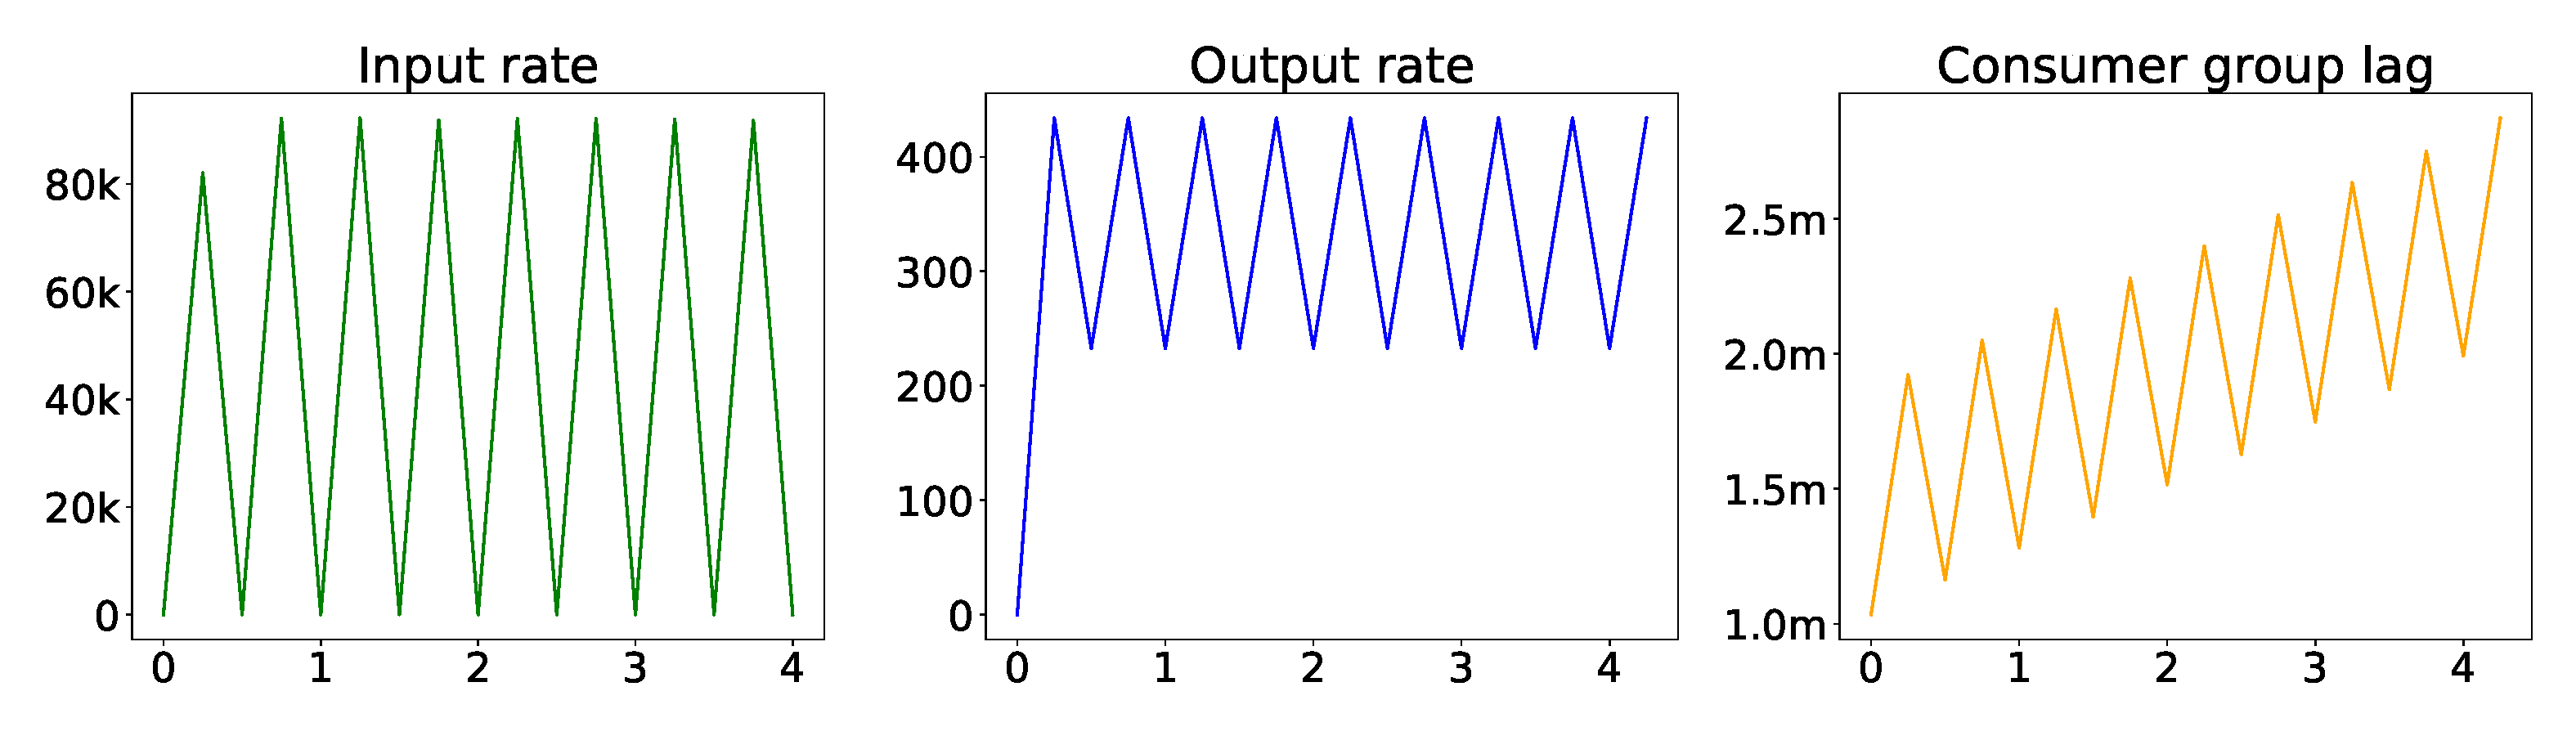
\includegraphics[width=1\textwidth]{figures/k-streams-java-21-new-gc-replicas-11}
    \caption{Benchmark parameters: input MPS = 50k, replicas = 11, selectivity = 0.00002, rules = 10000. \\
    Consumer group regression slope: 267264.}
    \label{fig:k-streams-java-21-new-gc-replicas-11}
\end{figure}

\begin{figure}[H]
    \centering
    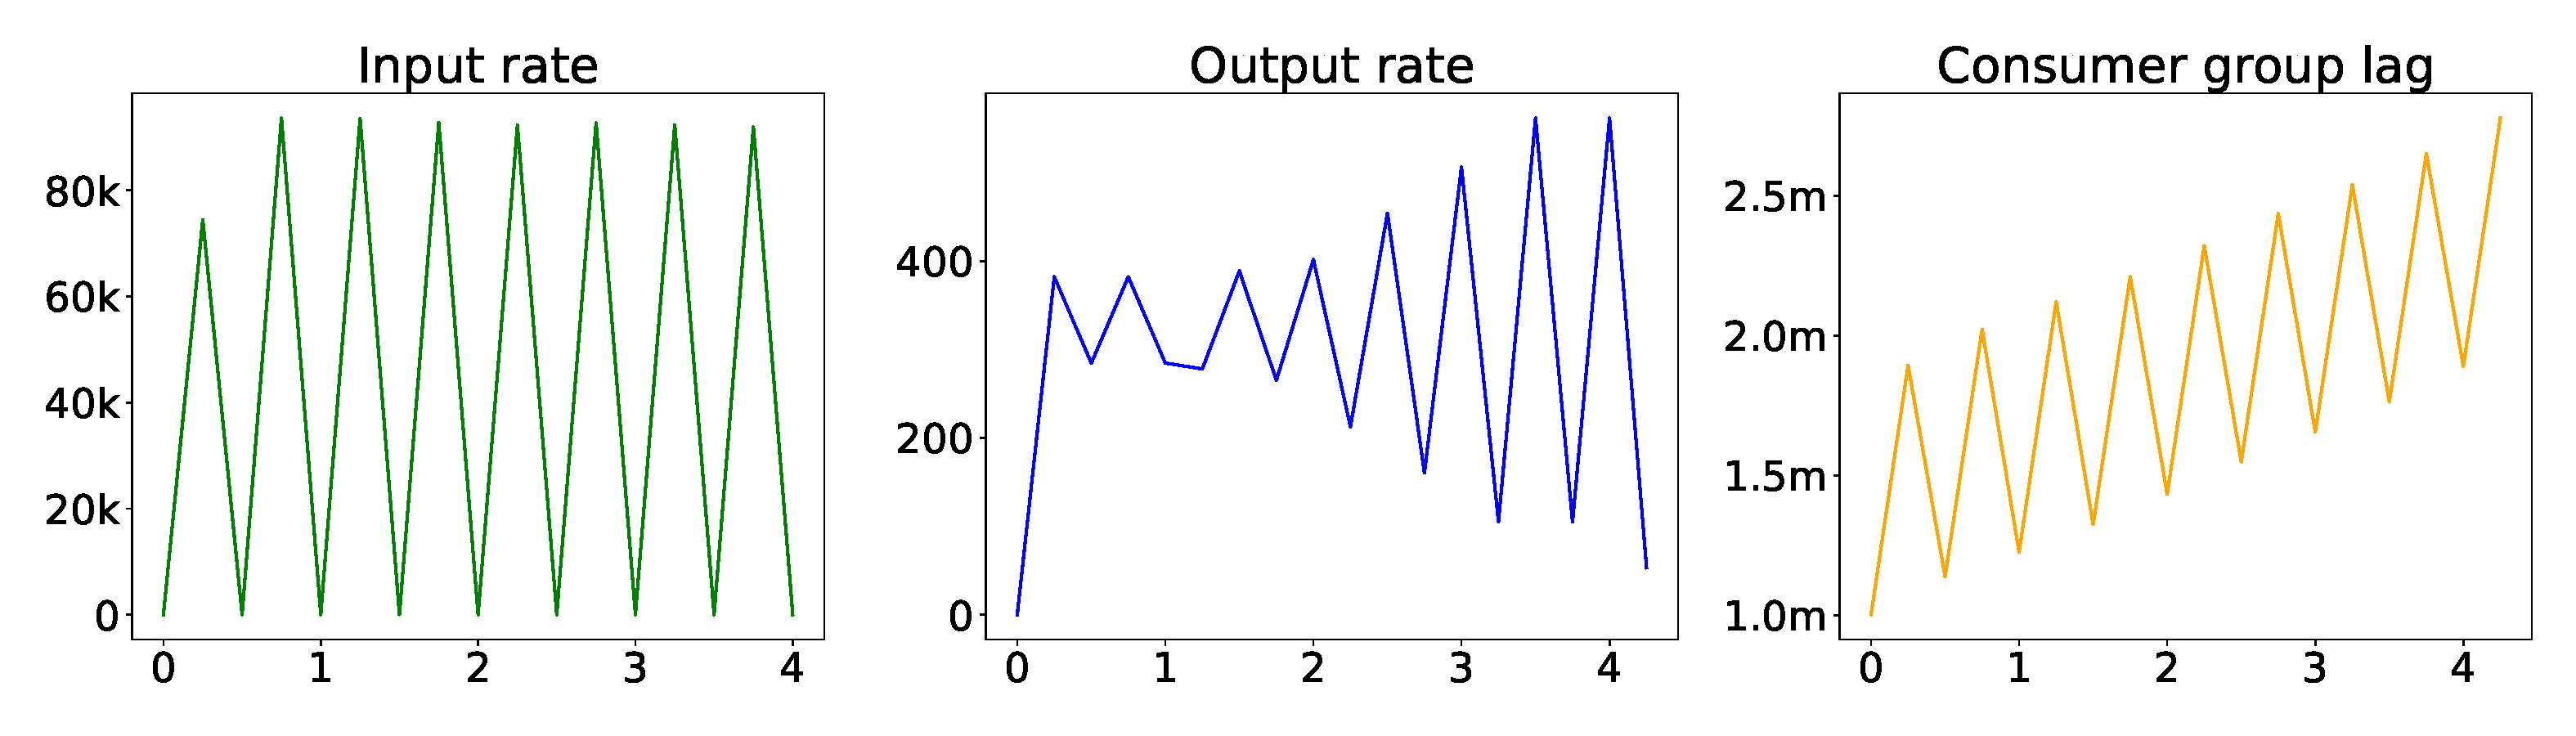
\includegraphics[width=1\textwidth]{figures/k-streams-java-21-new-gc-replicas-12}
    \caption{Benchmark parameters: input MPS = 50k, replicas = 12, selectivity = 0.00002, rules = 10000. \\
    Consumer group regression slope: 247516.}
    \label{fig:k-streams-java-21-new-gc-replicas-12}
\end{figure}


\newpage

\section{Flink on Java 11}\label{sec:flink-on-java-11}

\begin{figure}[H]
    \centering
    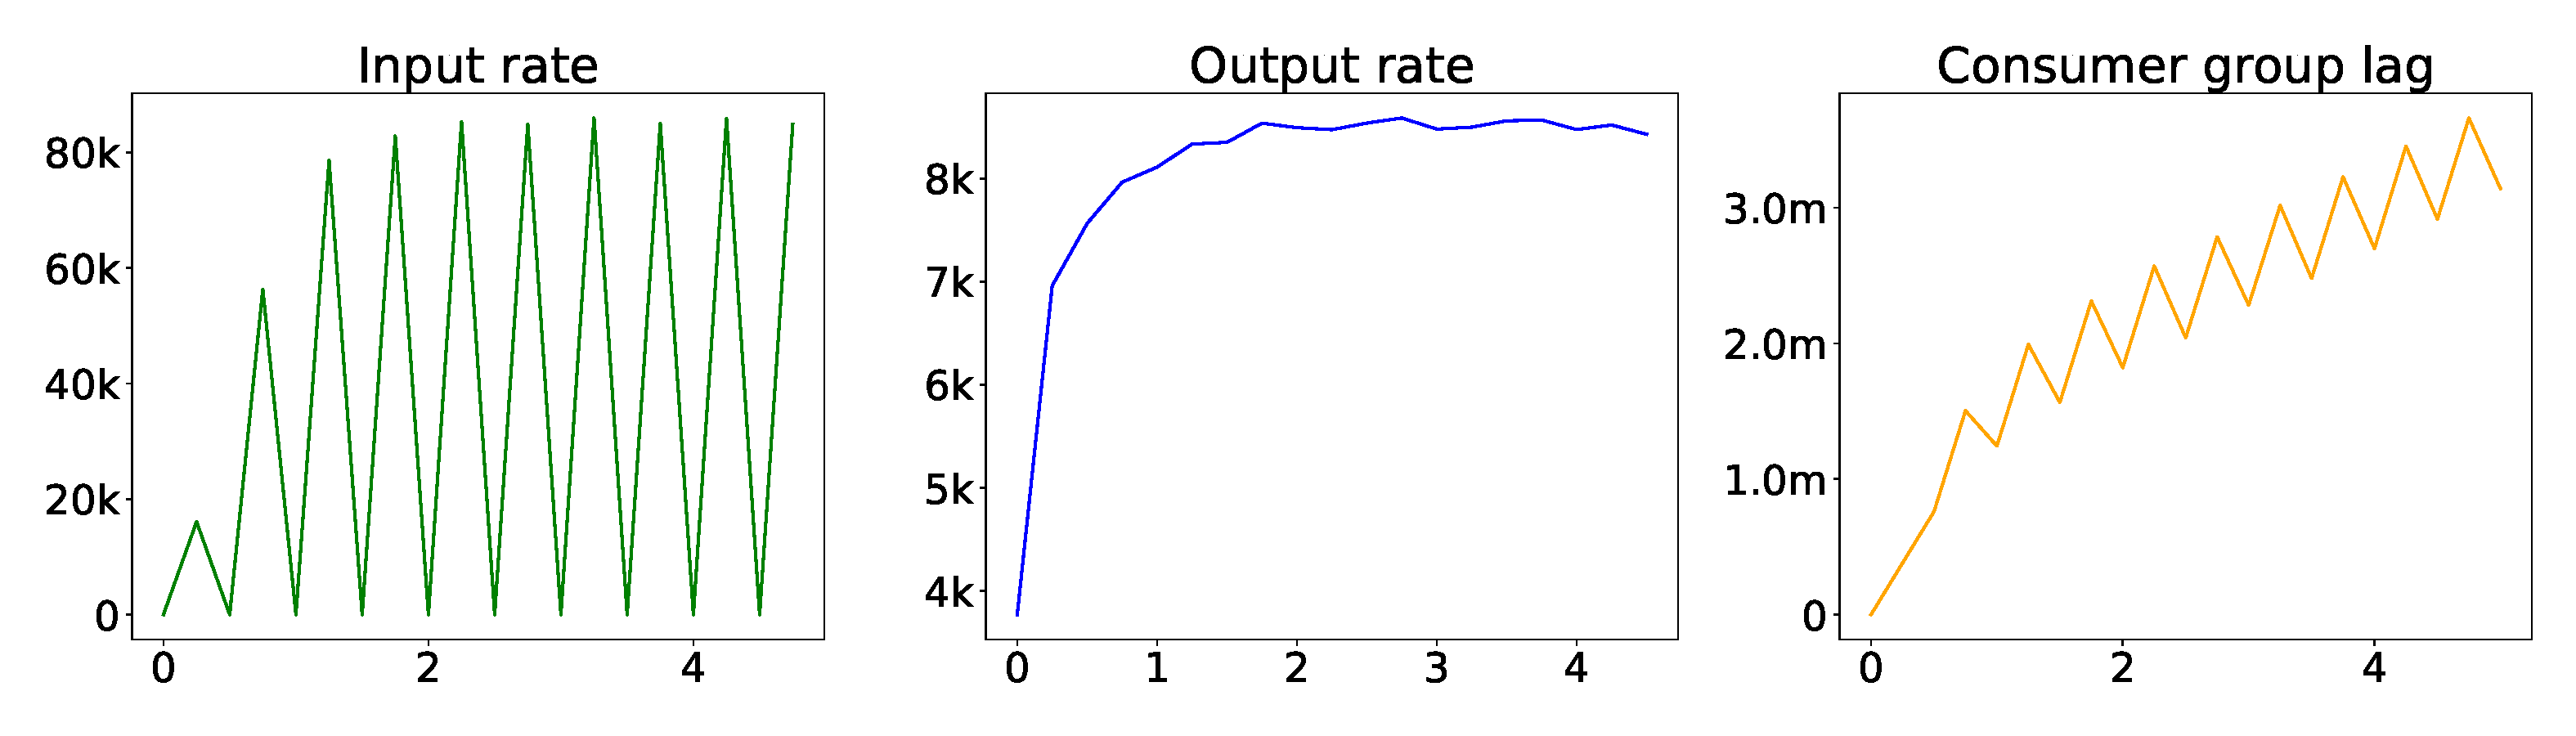
\includegraphics[width=1\textwidth]{figures/flink-java-11-replicas-10}
    \caption{Benchmark parameters: input MPS = 50k, replicas = 10, selectivity = 0.00002, rules = 10000. \\
    Consumer group regression slope: 463599.}
    \label{fig:flink-java-11-new-gc-replicas-10}
\end{figure}


\begin{figure}[H]
    \centering
    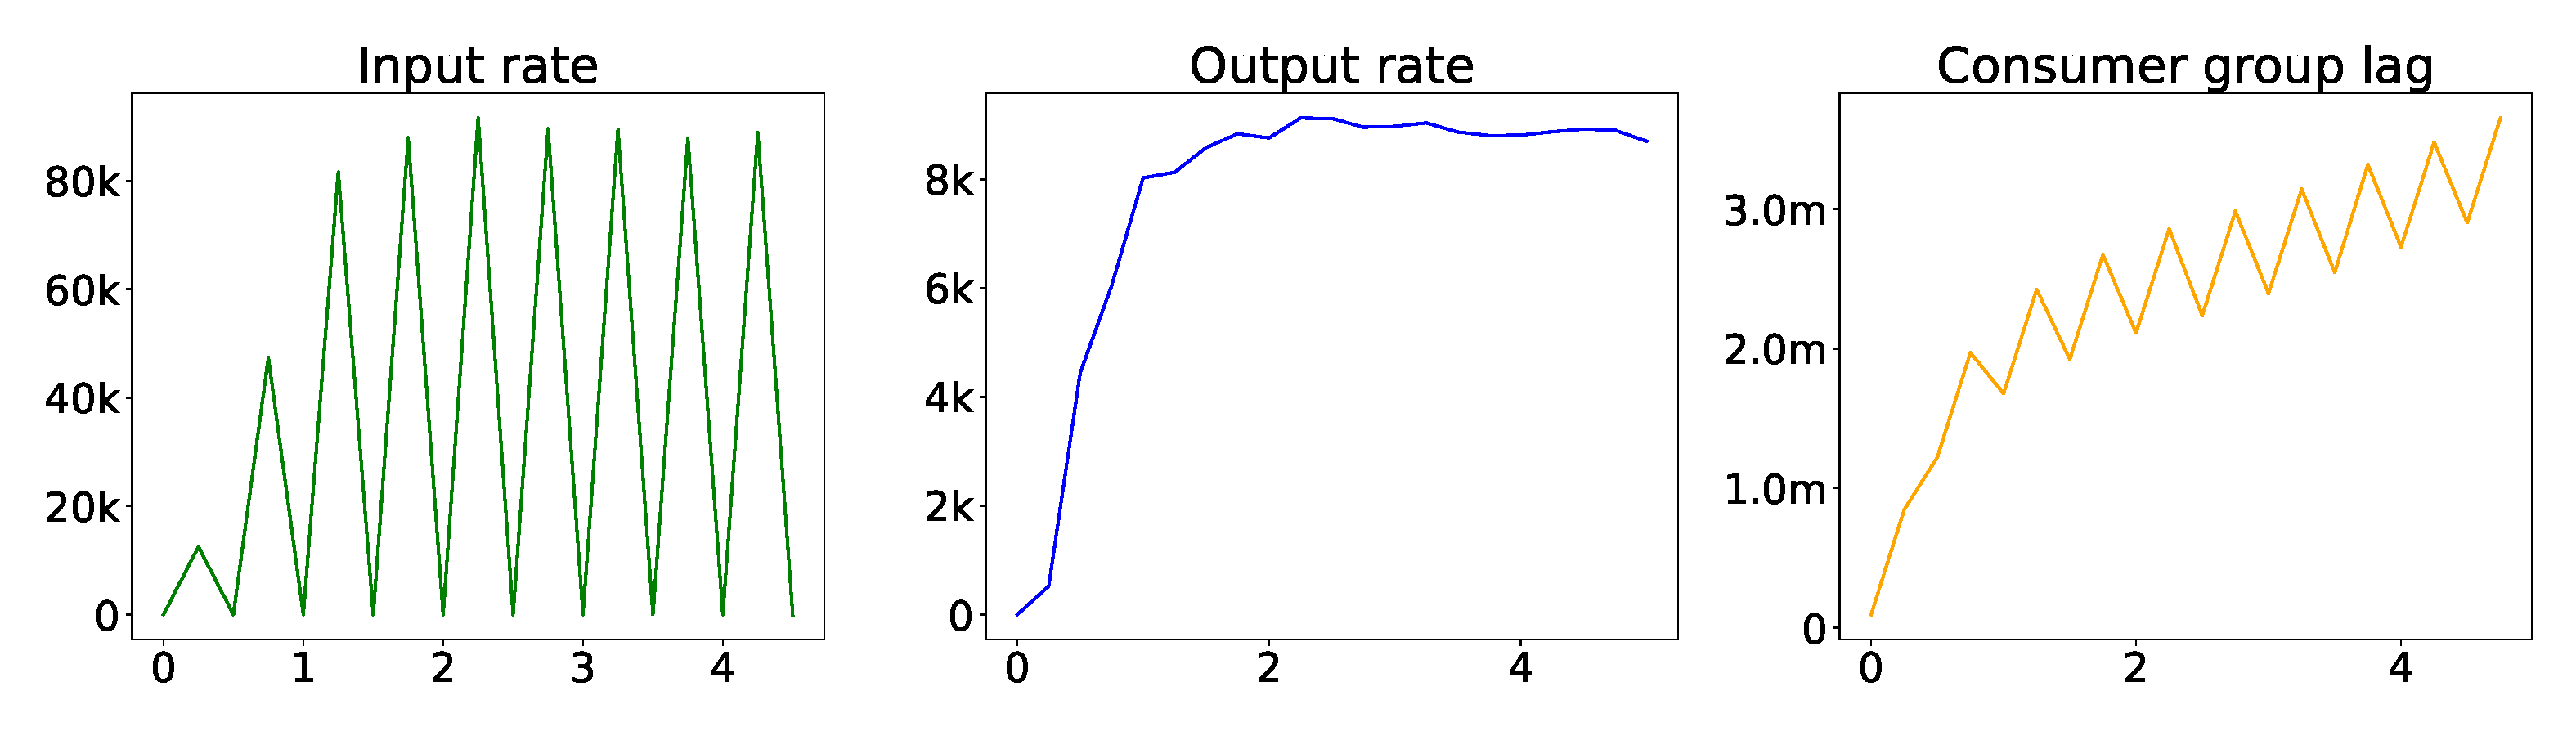
\includegraphics[width=1\textwidth]{figures/flink-java-11-replicas-11}
    \caption{Benchmark parameters: input MPS = 50k, replicas = 11, selectivity = 0.00002, rules = 10000. \\
    Consumer group regression slope: 367123.}
    \label{fig:flink-java-11-replicas-11}
\end{figure}

\begin{figure}[H]
    \centering
    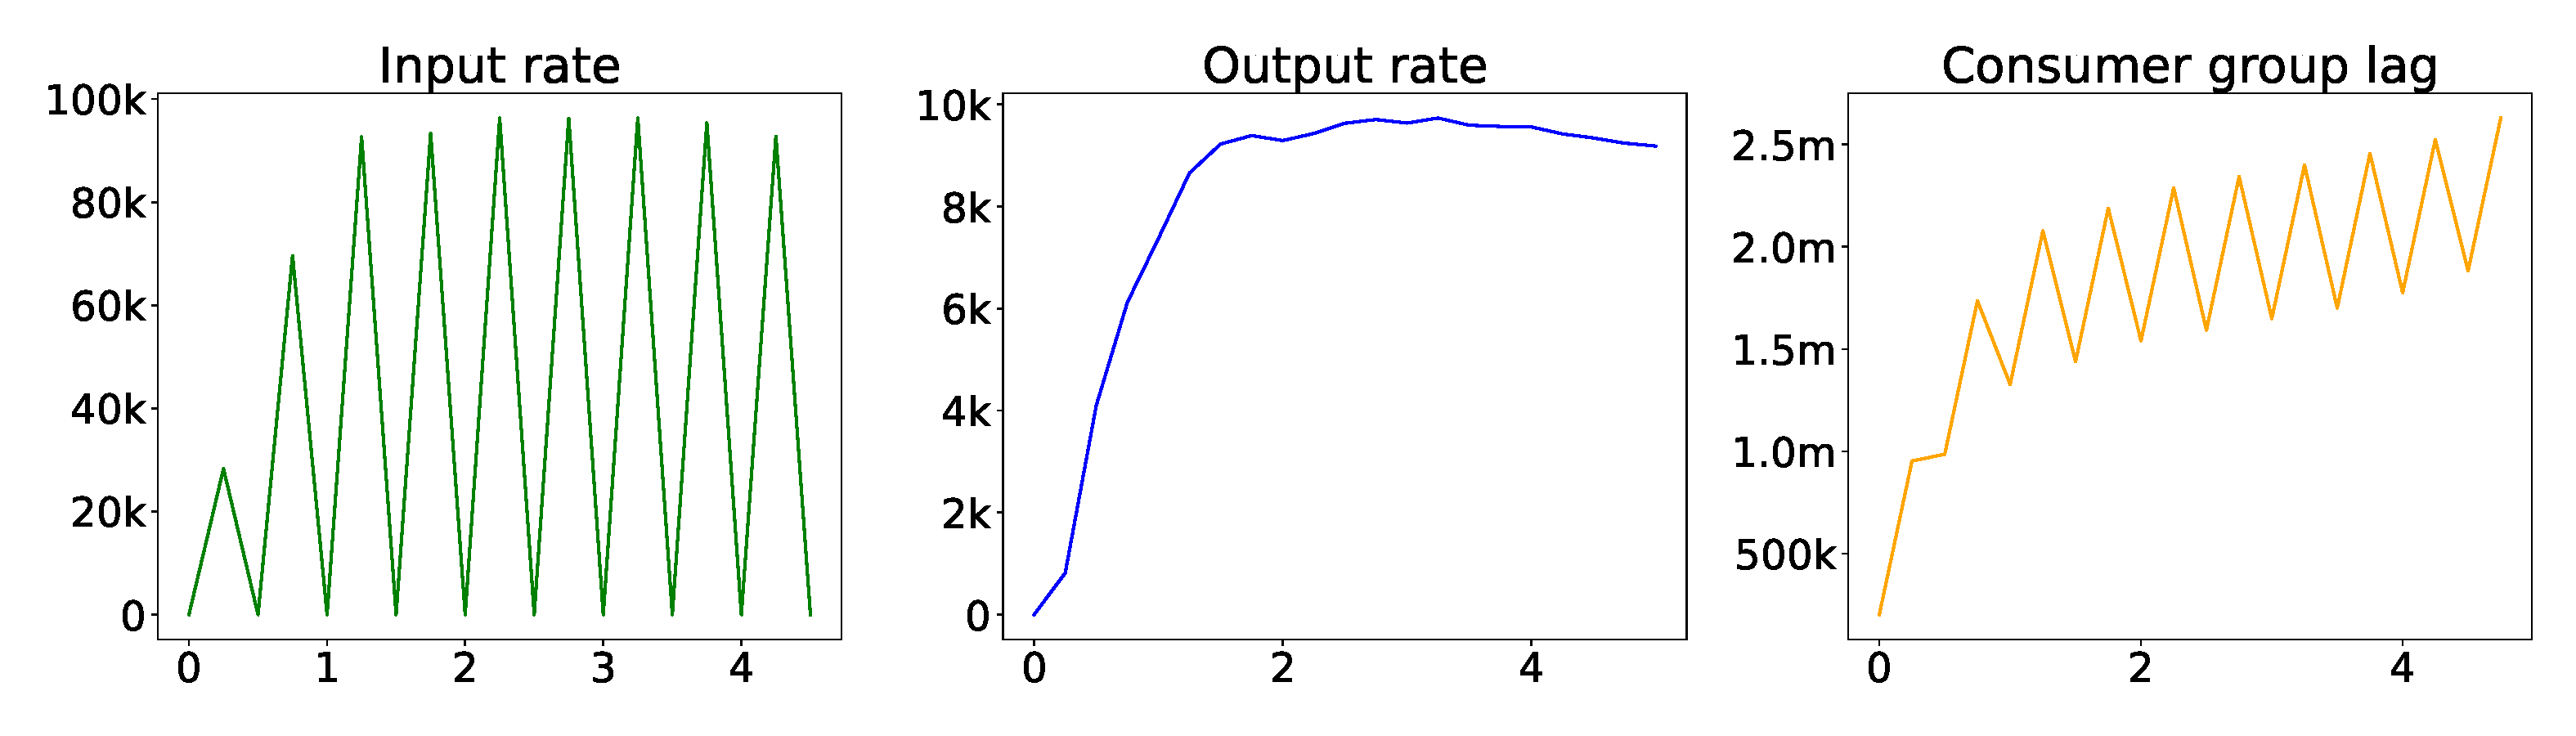
\includegraphics[width=1\textwidth]{figures/flink-java-11-replicas-12}
    \caption{Benchmark parameters: input MPS = 50k, replicas = 12, selectivity = 0.00002, rules = 10000. \\
    Consumer group regression slope: 178972.}
    \label{fig:flink-java-11-replicas-12}
\end{figure}


\newpage

\section{Flink on Java 21}\label{sec:flink-on-java-21}

\begin{figure}[H]
    \centering
    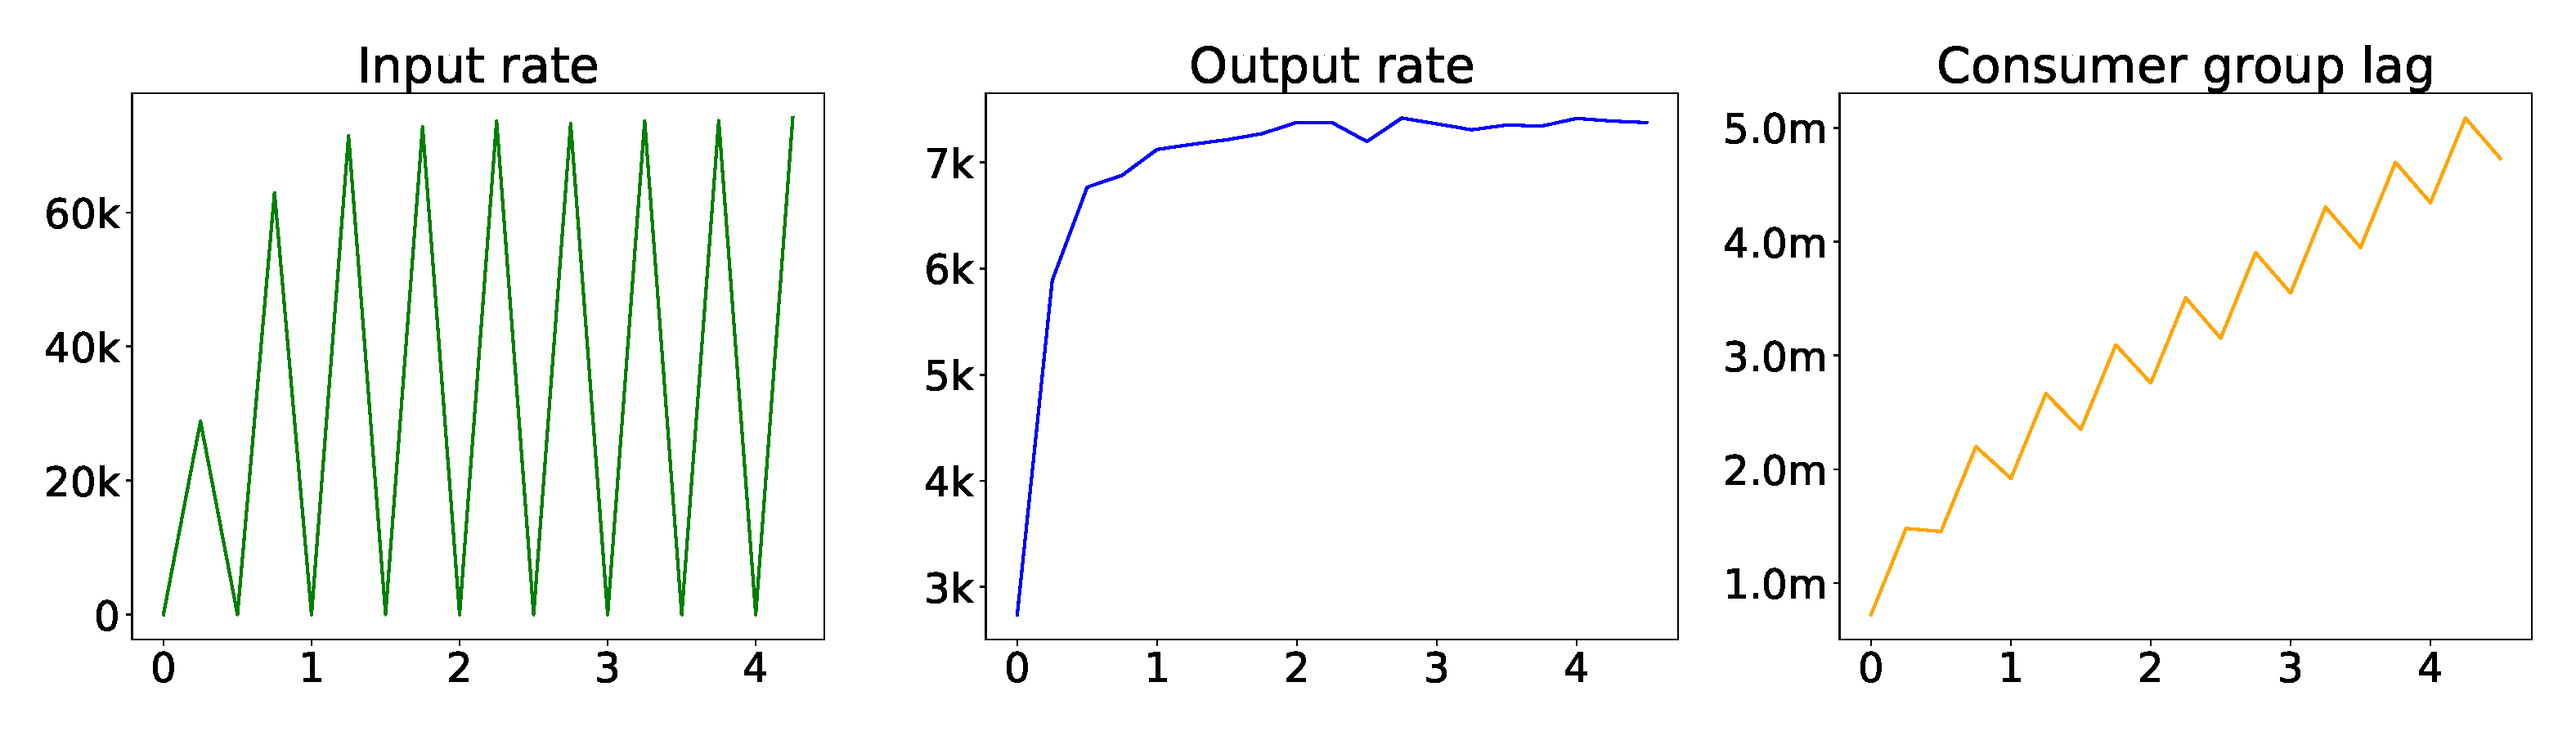
\includegraphics[width=1\textwidth]{figures/flink-java-21-replicas-10}
    \caption{Benchmark parameters: input MPS = 50k, replicas = 10, selectivity = 0.00002, rules = 10000. \\
    Consumer group regression slope: 802093.}
    \label{fig:flink-java-21-replicas-10}
\end{figure}


\begin{figure}[H]
    \centering
    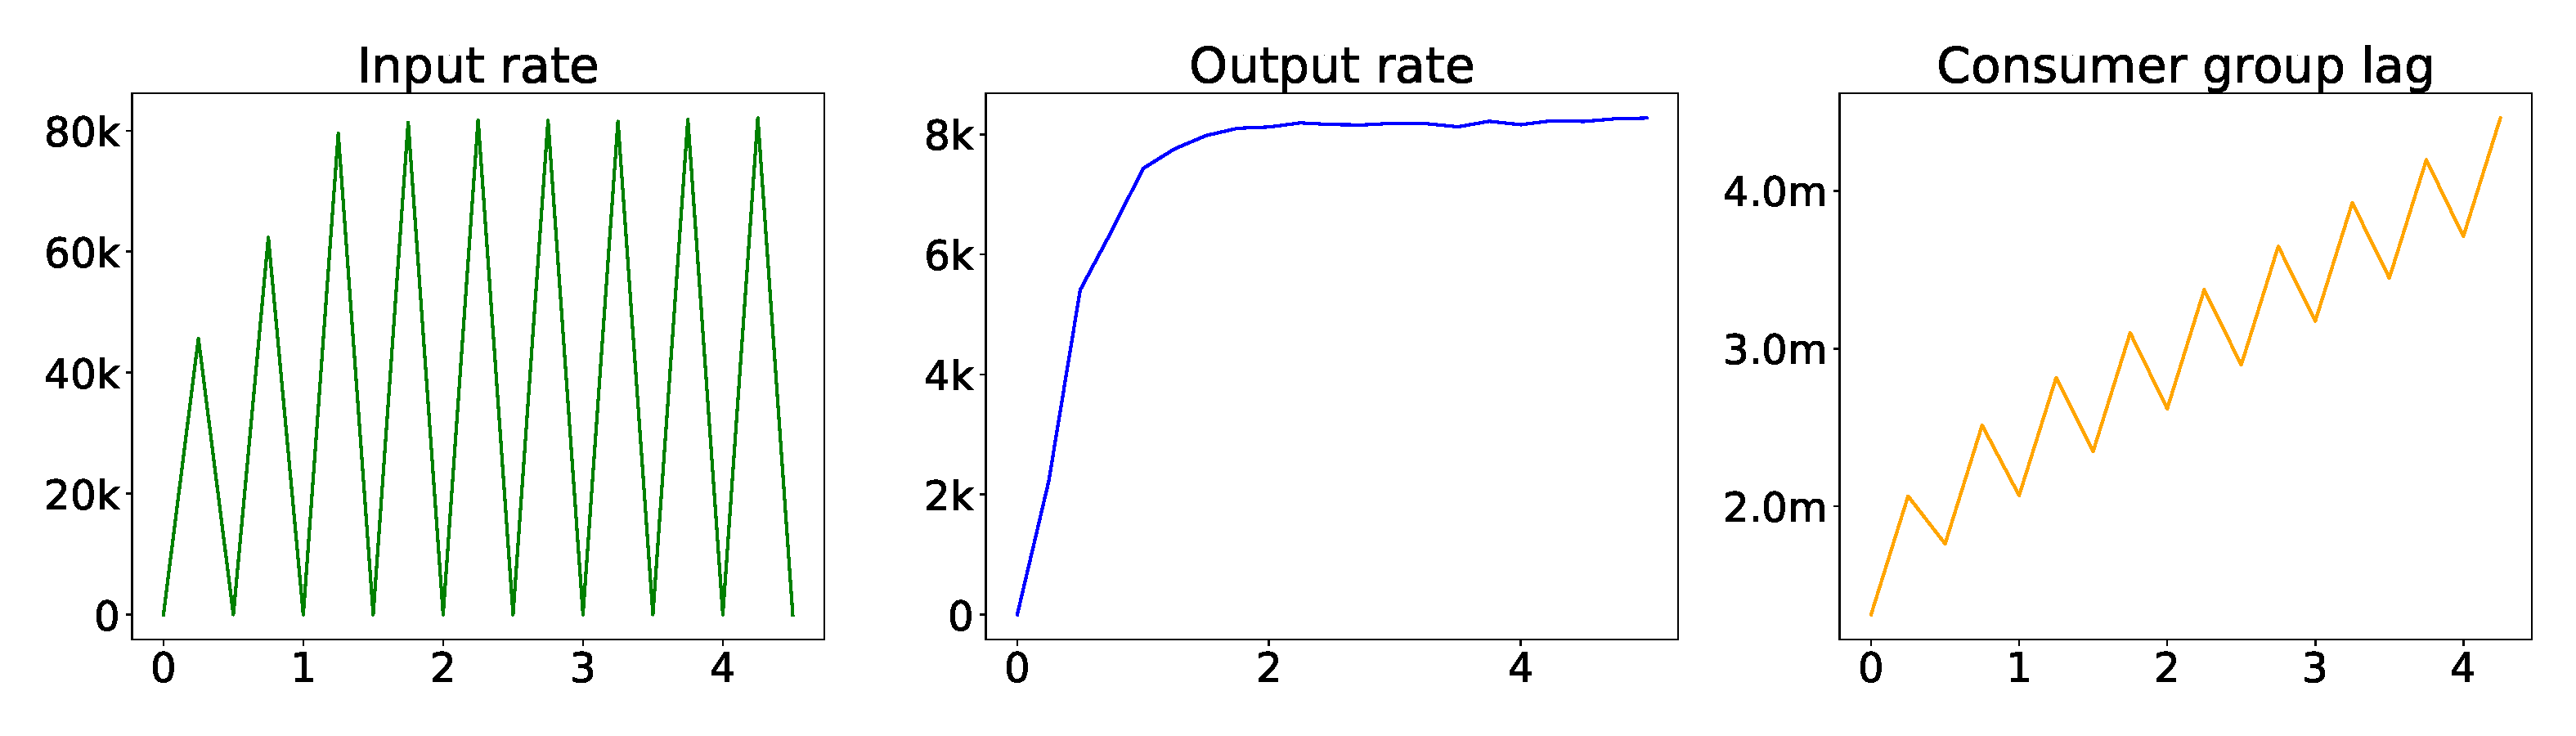
\includegraphics[width=1\textwidth]{figures/flink-java-21-replicas-11}
    \caption{Benchmark parameters: input MPS = 50k, replicas = 11, selectivity = 0.00002, rules = 10000. \\
    Consumer group regression slope: 586494.}
    \label{fig:flink-java-21-replicas-11}
\end{figure}

\begin{figure}[H]
    \centering
    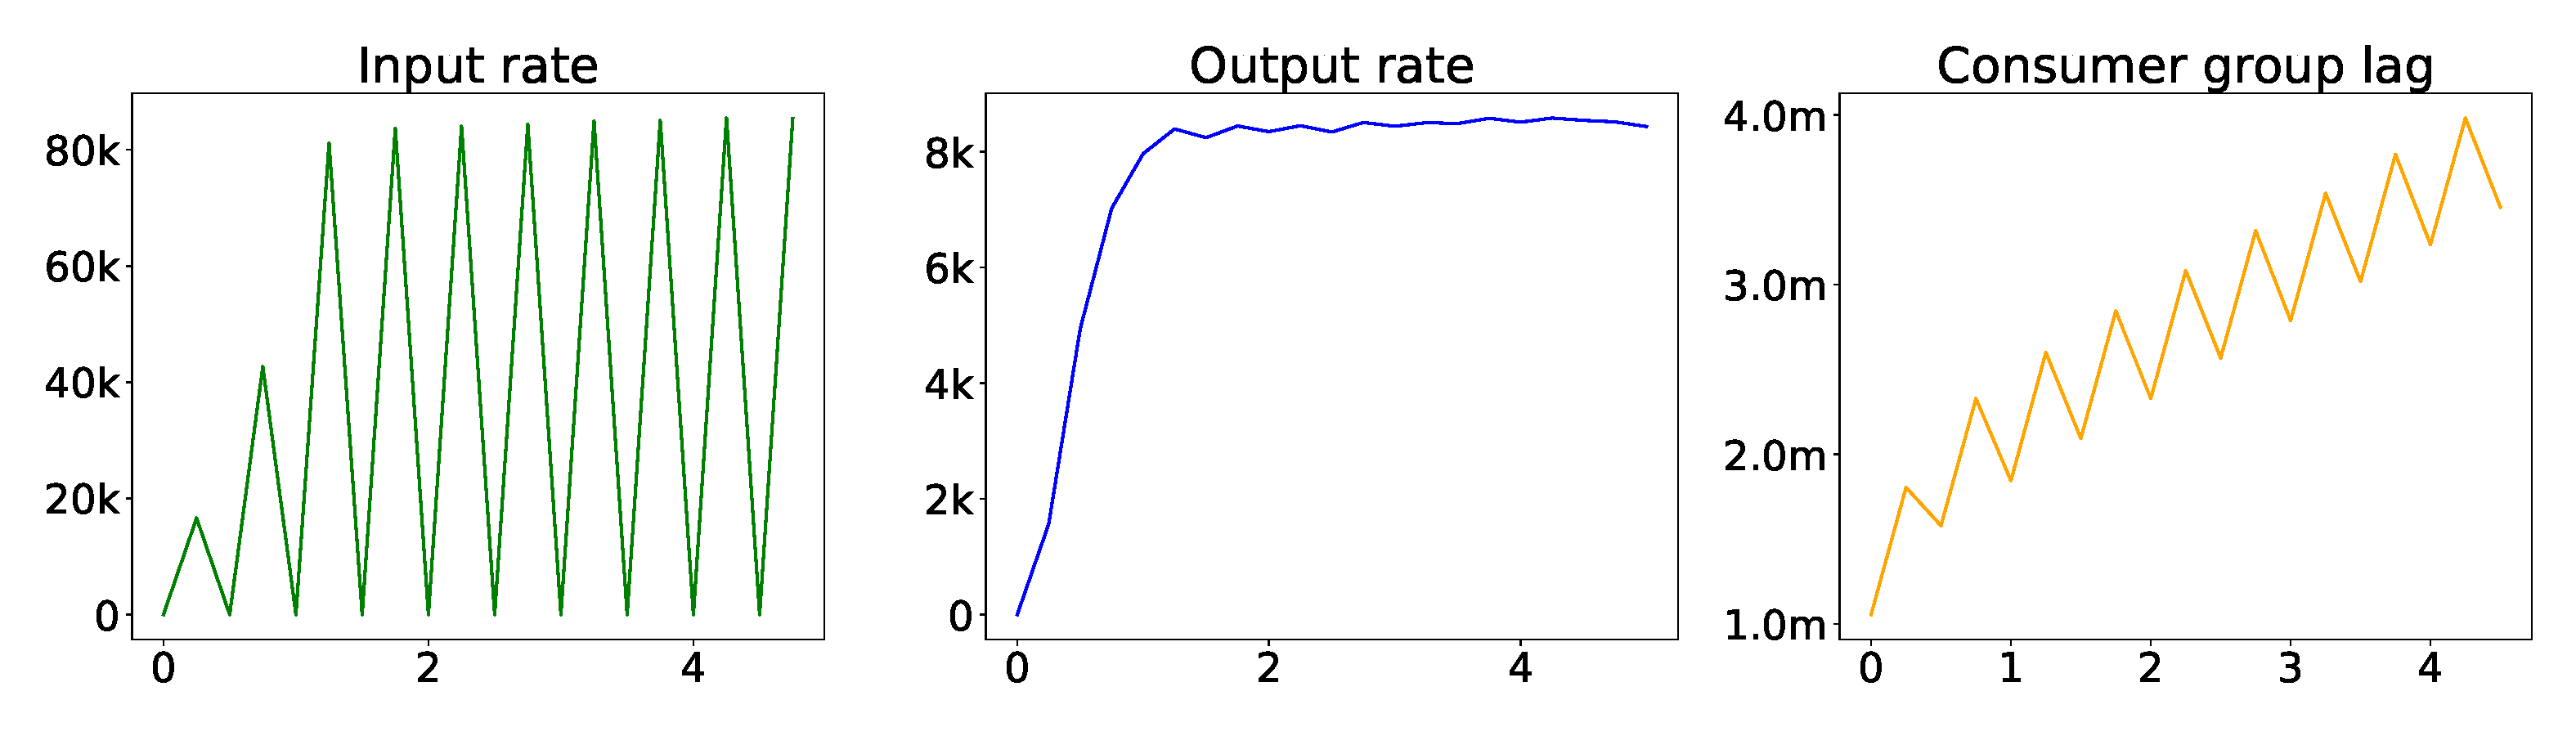
\includegraphics[width=1\textwidth]{figures/flink-java-21-replicas-12}
    \caption{Benchmark parameters: input MPS = 50k, replicas = 12, selectivity = 0.00002, rules = 10000. \\
    Consumer group regression slope: 459930.}
    \label{fig:flink-java-21-replicas-12}
\end{figure}


\newpage

\section{Flink on Java 21 with Generational ZGC}\label{sec:flink-on-java-21-with-generational-zgc}

\begin{figure}[H]
    \centering
    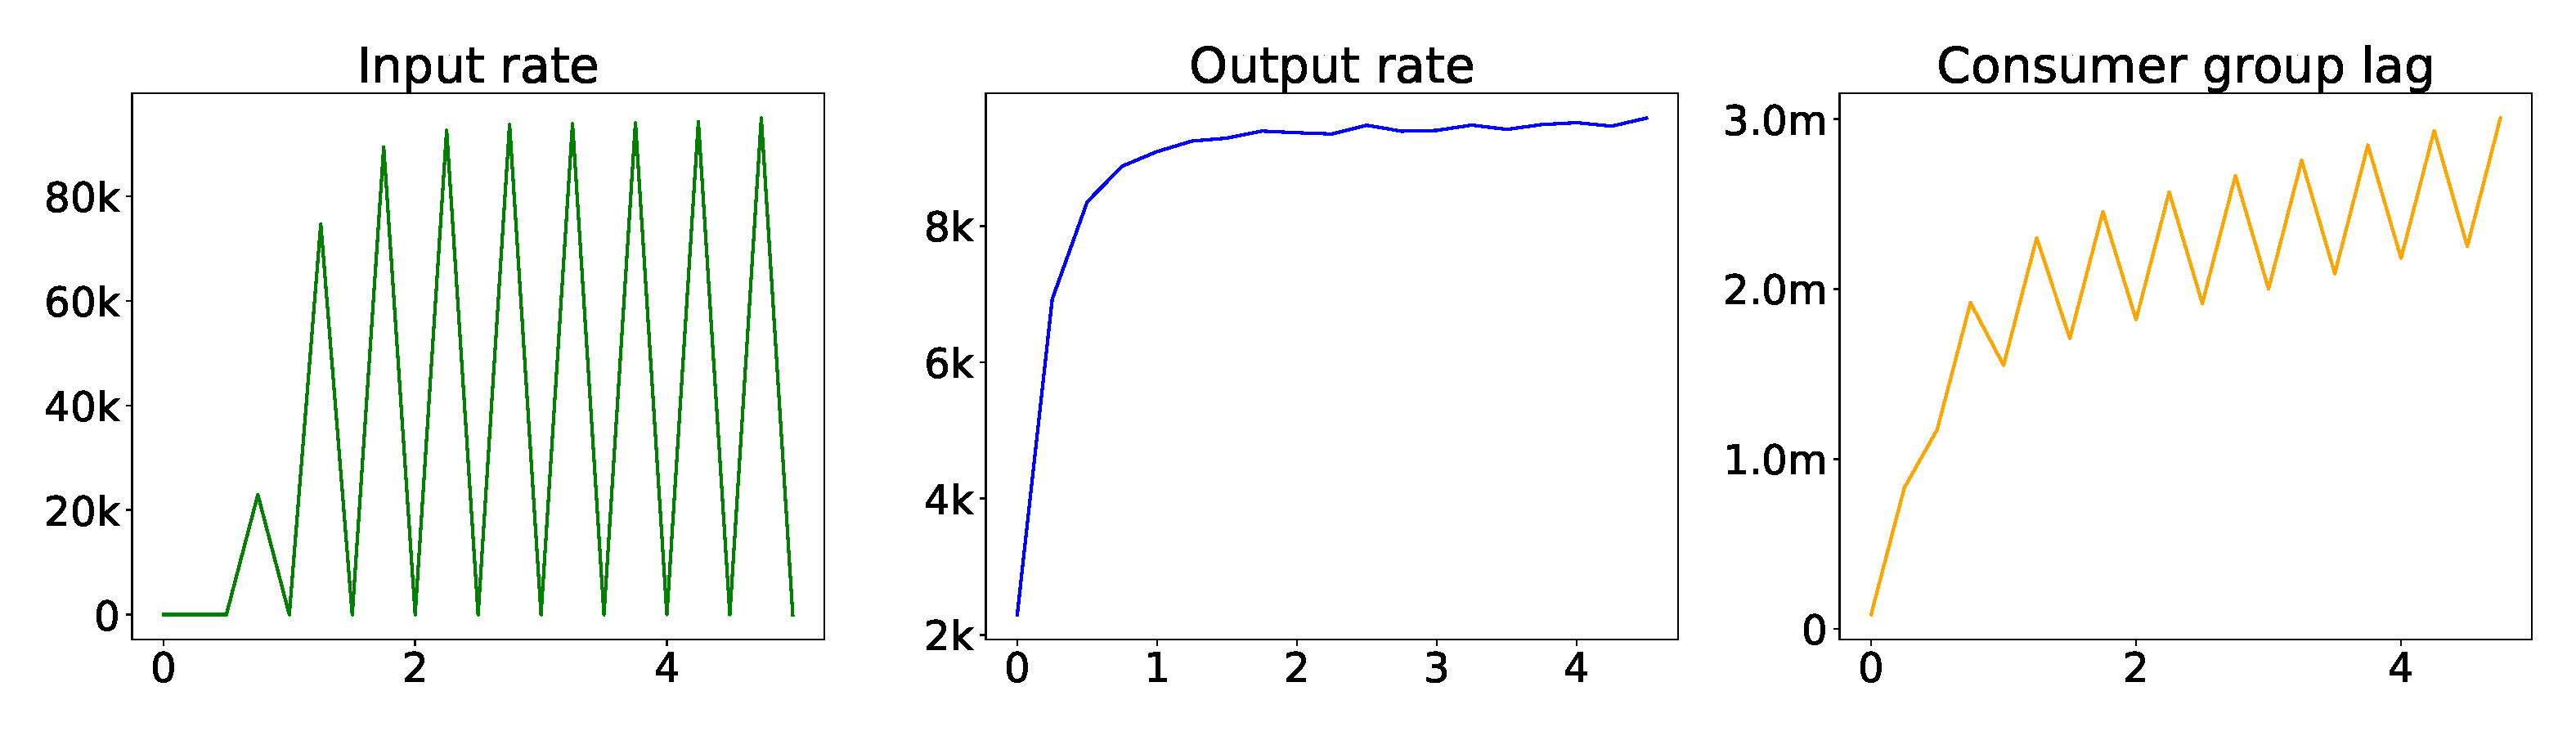
\includegraphics[width=1\textwidth]{figures/flink-java-21-new-gc-replicas-10}
    \caption{Benchmark parameters: input MPS = 50k, replicas = 10, selectivity = 0.00002, rules = 10000. \\
    Consumer group regression slope: 228068.}
    \label{fig:flink-java-21-new-gc-replicas-10}
\end{figure}

\begin{figure}[H]
    \centering
    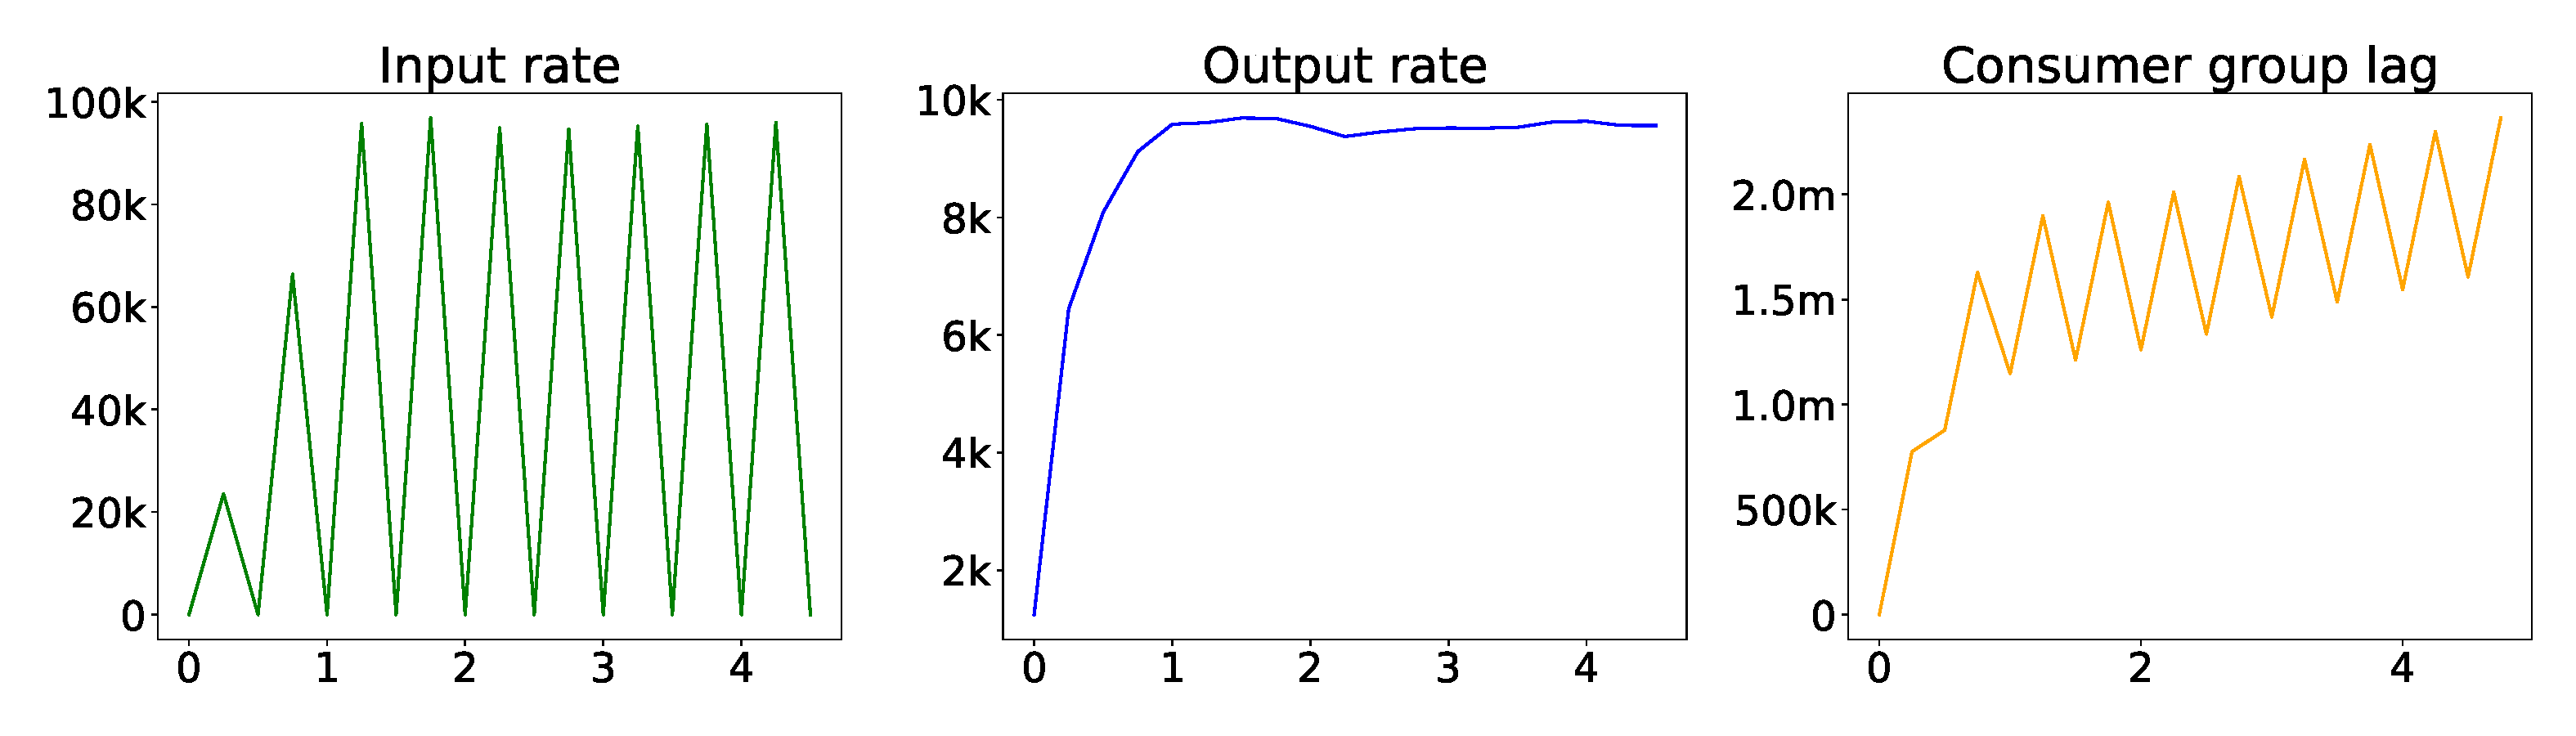
\includegraphics[width=1\textwidth]{figures/flink-java-21-new-gc-replicas-11}
    \caption{Benchmark parameters: input MPS = 50k, replicas = 11, selectivity = 0.00002, rules = 10000. \\
    Consumer group regression slope: 169020.}
    \label{fig:flink-java-21-new-gc-replicas-11}
\end{figure}

\begin{figure}[H]
    \centering
    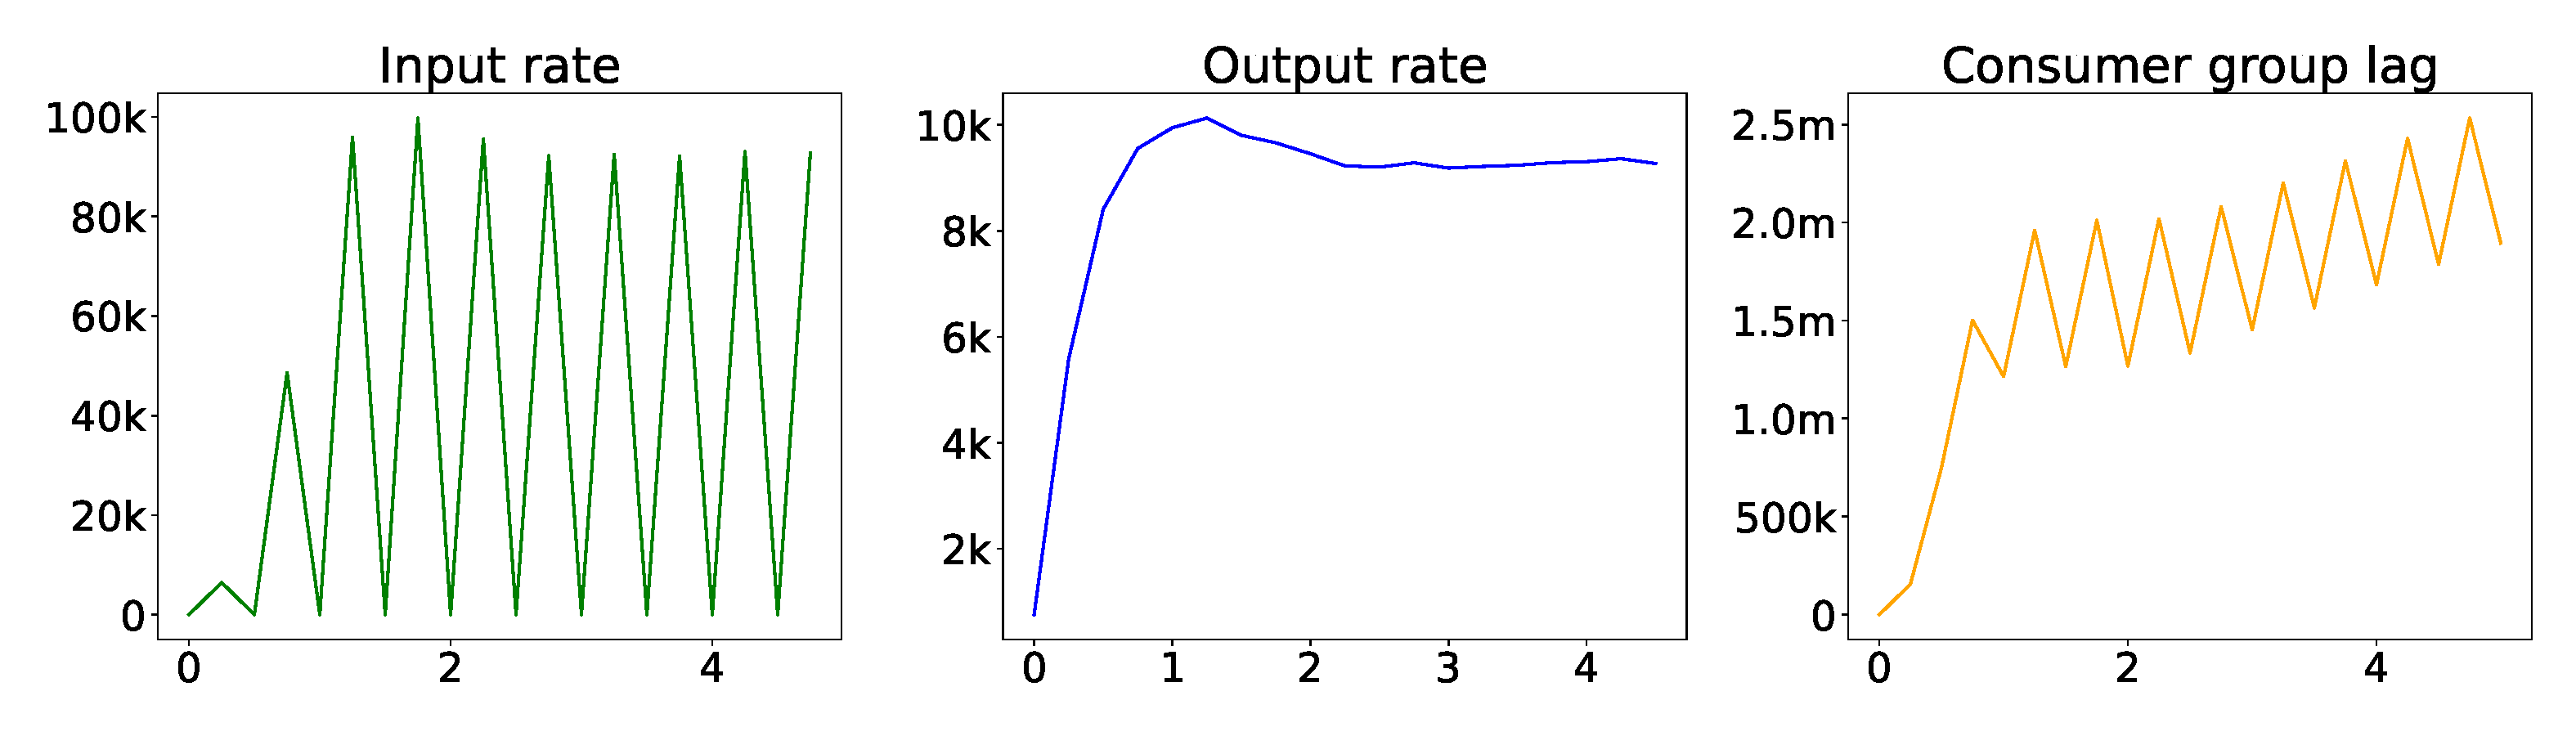
\includegraphics[width=1\textwidth]{figures/flink-java-21-new-gc-replicas-12}
    \caption{Benchmark parameters: input MPS = 50k, replicas = 12, selectivity = 0.00002, rules = 10000. \\
    Consumer group regression slope: 174466.}
    \label{fig:flink-java-21-new-gc-replicas-12}
\end{figure}



\section{Fault Tolerance}\label{sec:fault-tolerance}
During the following experiment 1 replica from 8 replicas gets killed to measure how the
system would react.

\begin{figure}[H]
    \centering
    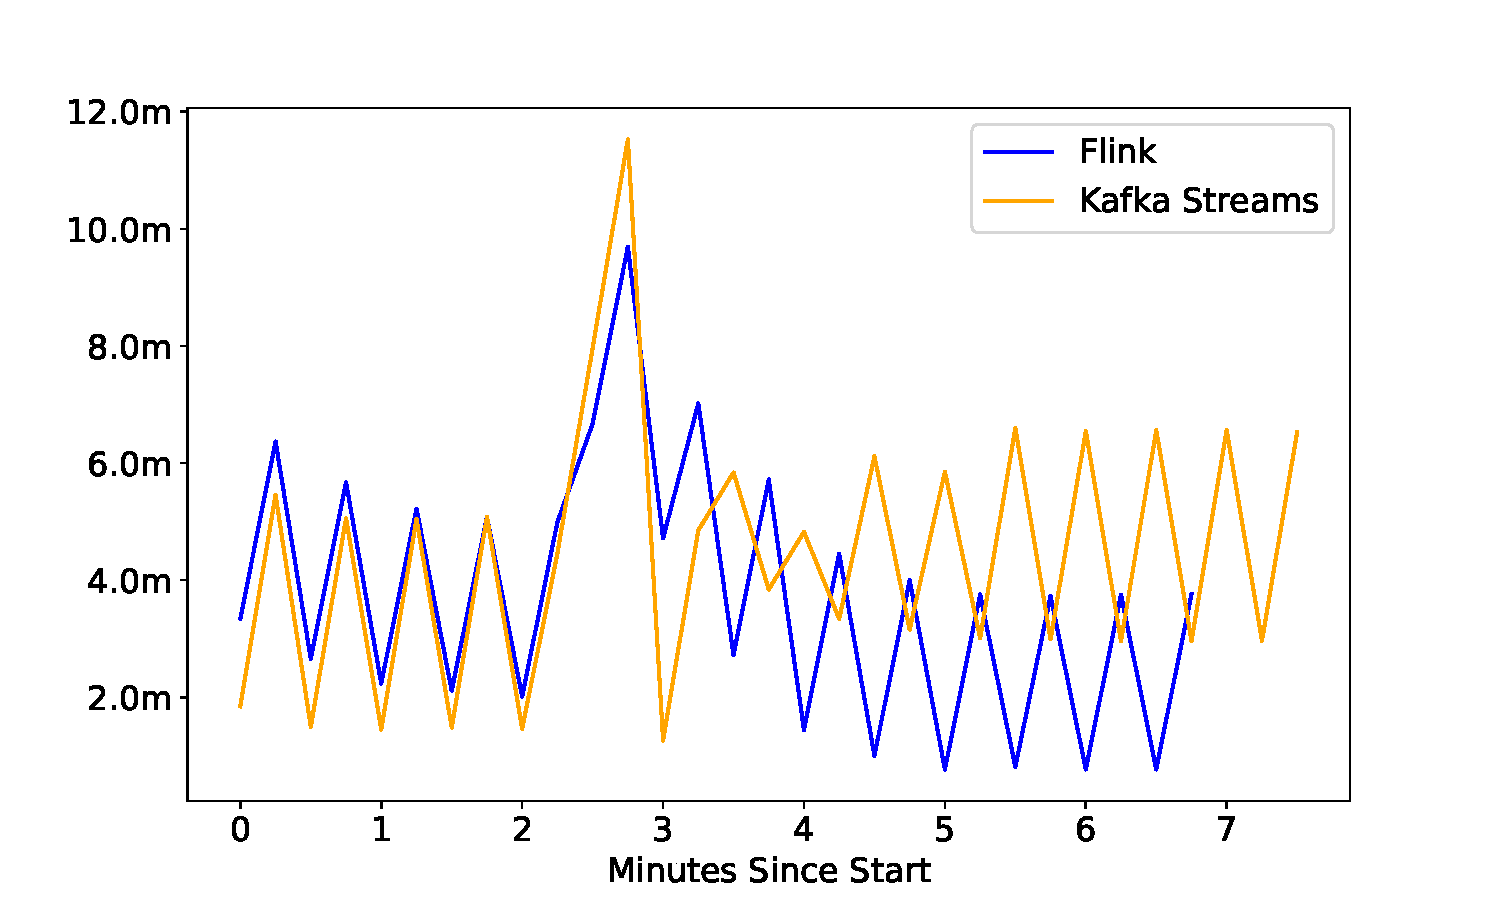
\includegraphics[width=1\textwidth]{figures/kafka-streams-flink-fault-tolerance}
    \caption{Benchmark parameters: input MPS = 200k, replicas = 8, selectivity = 0.0002, rules = 1000.}
    \label{fig:kafka-streams-flink-fault-tolerance}
\end{figure}
